\documentclass[]{book}
\usepackage{lmodern}
\usepackage{amssymb,amsmath}
\usepackage{ifxetex,ifluatex}
\usepackage{fixltx2e} % provides \textsubscript
\ifnum 0\ifxetex 1\fi\ifluatex 1\fi=0 % if pdftex
  \usepackage[T1]{fontenc}
  \usepackage[utf8]{inputenc}
\else % if luatex or xelatex
  \ifxetex
    \usepackage{mathspec}
  \else
    \usepackage{fontspec}
  \fi
  \defaultfontfeatures{Ligatures=TeX,Scale=MatchLowercase}
\fi
% use upquote if available, for straight quotes in verbatim environments
\IfFileExists{upquote.sty}{\usepackage{upquote}}{}
% use microtype if available
\IfFileExists{microtype.sty}{%
\usepackage{microtype}
\UseMicrotypeSet[protrusion]{basicmath} % disable protrusion for tt fonts
}{}
\usepackage[margin=1in]{geometry}
\usepackage{hyperref}
\hypersetup{unicode=true,
            pdftitle={Applied SNA with R},
            pdfauthor={George G. Vega Yon},
            pdfborder={0 0 0},
            breaklinks=true}
\urlstyle{same}  % don't use monospace font for urls
\usepackage{color}
\usepackage{fancyvrb}
\newcommand{\VerbBar}{|}
\newcommand{\VERB}{\Verb[commandchars=\\\{\}]}
\DefineVerbatimEnvironment{Highlighting}{Verbatim}{commandchars=\\\{\}}
% Add ',fontsize=\small' for more characters per line
\usepackage{framed}
\definecolor{shadecolor}{RGB}{248,248,248}
\newenvironment{Shaded}{\begin{snugshade}}{\end{snugshade}}
\newcommand{\KeywordTok}[1]{\textcolor[rgb]{0.13,0.29,0.53}{\textbf{#1}}}
\newcommand{\DataTypeTok}[1]{\textcolor[rgb]{0.13,0.29,0.53}{#1}}
\newcommand{\DecValTok}[1]{\textcolor[rgb]{0.00,0.00,0.81}{#1}}
\newcommand{\BaseNTok}[1]{\textcolor[rgb]{0.00,0.00,0.81}{#1}}
\newcommand{\FloatTok}[1]{\textcolor[rgb]{0.00,0.00,0.81}{#1}}
\newcommand{\ConstantTok}[1]{\textcolor[rgb]{0.00,0.00,0.00}{#1}}
\newcommand{\CharTok}[1]{\textcolor[rgb]{0.31,0.60,0.02}{#1}}
\newcommand{\SpecialCharTok}[1]{\textcolor[rgb]{0.00,0.00,0.00}{#1}}
\newcommand{\StringTok}[1]{\textcolor[rgb]{0.31,0.60,0.02}{#1}}
\newcommand{\VerbatimStringTok}[1]{\textcolor[rgb]{0.31,0.60,0.02}{#1}}
\newcommand{\SpecialStringTok}[1]{\textcolor[rgb]{0.31,0.60,0.02}{#1}}
\newcommand{\ImportTok}[1]{#1}
\newcommand{\CommentTok}[1]{\textcolor[rgb]{0.56,0.35,0.01}{\textit{#1}}}
\newcommand{\DocumentationTok}[1]{\textcolor[rgb]{0.56,0.35,0.01}{\textbf{\textit{#1}}}}
\newcommand{\AnnotationTok}[1]{\textcolor[rgb]{0.56,0.35,0.01}{\textbf{\textit{#1}}}}
\newcommand{\CommentVarTok}[1]{\textcolor[rgb]{0.56,0.35,0.01}{\textbf{\textit{#1}}}}
\newcommand{\OtherTok}[1]{\textcolor[rgb]{0.56,0.35,0.01}{#1}}
\newcommand{\FunctionTok}[1]{\textcolor[rgb]{0.00,0.00,0.00}{#1}}
\newcommand{\VariableTok}[1]{\textcolor[rgb]{0.00,0.00,0.00}{#1}}
\newcommand{\ControlFlowTok}[1]{\textcolor[rgb]{0.13,0.29,0.53}{\textbf{#1}}}
\newcommand{\OperatorTok}[1]{\textcolor[rgb]{0.81,0.36,0.00}{\textbf{#1}}}
\newcommand{\BuiltInTok}[1]{#1}
\newcommand{\ExtensionTok}[1]{#1}
\newcommand{\PreprocessorTok}[1]{\textcolor[rgb]{0.56,0.35,0.01}{\textit{#1}}}
\newcommand{\AttributeTok}[1]{\textcolor[rgb]{0.77,0.63,0.00}{#1}}
\newcommand{\RegionMarkerTok}[1]{#1}
\newcommand{\InformationTok}[1]{\textcolor[rgb]{0.56,0.35,0.01}{\textbf{\textit{#1}}}}
\newcommand{\WarningTok}[1]{\textcolor[rgb]{0.56,0.35,0.01}{\textbf{\textit{#1}}}}
\newcommand{\AlertTok}[1]{\textcolor[rgb]{0.94,0.16,0.16}{#1}}
\newcommand{\ErrorTok}[1]{\textcolor[rgb]{0.64,0.00,0.00}{\textbf{#1}}}
\newcommand{\NormalTok}[1]{#1}
\usepackage{longtable,booktabs}
\usepackage{graphicx,grffile}
\makeatletter
\def\maxwidth{\ifdim\Gin@nat@width>\linewidth\linewidth\else\Gin@nat@width\fi}
\def\maxheight{\ifdim\Gin@nat@height>\textheight\textheight\else\Gin@nat@height\fi}
\makeatother
% Scale images if necessary, so that they will not overflow the page
% margins by default, and it is still possible to overwrite the defaults
% using explicit options in \includegraphics[width, height, ...]{}
\setkeys{Gin}{width=\maxwidth,height=\maxheight,keepaspectratio}
\IfFileExists{parskip.sty}{%
\usepackage{parskip}
}{% else
\setlength{\parindent}{0pt}
\setlength{\parskip}{6pt plus 2pt minus 1pt}
}
\setlength{\emergencystretch}{3em}  % prevent overfull lines
\providecommand{\tightlist}{%
  \setlength{\itemsep}{0pt}\setlength{\parskip}{0pt}}
\setcounter{secnumdepth}{5}
% Redefines (sub)paragraphs to behave more like sections
\ifx\paragraph\undefined\else
\let\oldparagraph\paragraph
\renewcommand{\paragraph}[1]{\oldparagraph{#1}\mbox{}}
\fi
\ifx\subparagraph\undefined\else
\let\oldsubparagraph\subparagraph
\renewcommand{\subparagraph}[1]{\oldsubparagraph{#1}\mbox{}}
\fi

%%% Use protect on footnotes to avoid problems with footnotes in titles
\let\rmarkdownfootnote\footnote%
\def\footnote{\protect\rmarkdownfootnote}

%%% Change title format to be more compact
\usepackage{titling}

% Create subtitle command for use in maketitle
\newcommand{\subtitle}[1]{
  \posttitle{
    \begin{center}\large#1\end{center}
    }
}

\setlength{\droptitle}{-2em}
  \title{Applied SNA with R}
  \pretitle{\vspace{\droptitle}\centering\huge}
  \posttitle{\par}
  \author{George G. Vega Yon}
  \preauthor{\centering\large\emph}
  \postauthor{\par}
  \predate{\centering\large\emph}
  \postdate{\par}
  \date{2018-03-12}

\usepackage{booktabs}
\usepackage{hyperref}
  \hypersetup{allcolors=blue, colorlinks=true}

\usepackage{setspace}
\doublespacing

\usepackage{arev}
\usepackage[T1]{fontenc}

\usepackage{amsthm}
\newtheorem{theorem}{Theorem}[chapter]
\newtheorem{lemma}{Lemma}[chapter]
\theoremstyle{definition}
\newtheorem{definition}{Definition}[chapter]
\newtheorem{corollary}{Corollary}[chapter]
\newtheorem{proposition}{Proposition}[chapter]
\theoremstyle{definition}
\newtheorem{example}{Example}[chapter]
\theoremstyle{definition}
\newtheorem{exercise}{Exercise}[chapter]
\theoremstyle{remark}
\newtheorem*{remark}{Remark}
\newtheorem*{solution}{Solution}
\begin{document}
\maketitle

{
\setcounter{tocdepth}{1}
\tableofcontents
}
\renewcommand{\Pr}[1]{\mbox{Pr}\left(#1\right)}
\renewcommand{\exp}[1]{\mbox{exp}\left\{#1\right\}}

\chapter{About this book}\label{about-this-book}

This book will be build as part of a workshop on Applied Social Network
Analysis with R. Its contents will be populated as the sessions take
place, and for now there is particular program that we will follow,
instead, we have the following workflow:

\begin{enumerate}
\def\labelenumi{\arabic{enumi}.}
\item
  Participants will share their data and what they need to do with it.
\item
  Based on their data, I'll be preparing the sessions trying to show
  attendees how would I approach the problem, and at the same time,
  teach by example about the R language.
\item
  Materials will be published on this website and, hopefully, video
  recordings of the sessions.
\end{enumerate}

At least in the first version, the book will be organized by session,
this is, one chapter per session.

All the book materials can be downloaded from
\url{https://github.com/gvegayon/appliedsnar}

In general, we will besides of R itself, we will be using R studio and
the following R packages: dplyr for data management, stringr for data
cleaning, and of course igraph, netdiffuseR (a bit of a bias here), and
statnet for our neat network analysis.\footnote{Some of you may be
  wondering ``what about ggplot2 and friends? What about
  \href{https://www.tidyverse.org/}{\texttt{tidyverse}}'', well, my
  short answer is I jumped into R before all of that was that popular.
  When I started plots were all about
  \href{https://CRAN.R-project.org/package=lattice}{\texttt{lattice}},
  and after a couple of years on that, about base R graphics. What I'm
  saying is that so far I have not find a compelling reason to leave my
  ``old-practices'' and embrace all the \texttt{tidyverse} movement
  (religion?).}

\chapter{Introduction}\label{introduction}

For this book we need the following

\begin{enumerate}
\def\labelenumi{\arabic{enumi}.}
\item
  Install R from CRAN: \url{https://www.r-project.org/}
\item
  (optional) Install Rstudio: \url{https://rstudio.org}
\end{enumerate}

While I find RStudio extreamly useful, it is not necesary to use it with
R.

\chapter{R Basics}\label{r-basics}

\section{What is R}\label{what-is-r}

A good reference book for both new and advanced user is
\href{https://nostarch.com/artofr.htm}{``The Art of R programming''}
(Matloff \protect\hyperlink{ref-Matloff2011}{2011})\footnote{\href{http://heather.cs.ucdavis.edu/~matloff/145/PLN/RMaterials/NSPpart.pdf}{Here}
  a free pdf version distributed by the author.}

\section{How to install packages}\label{how-to-install-packages}

Nowadays there are two ways of installing R packages (that I'm aware
of), either using \texttt{install.packages}, which is a function shipped
with R, or use the devtools R package to install a package from some
remote repository other than CRAN, here is a couple of examples:

\begin{Shaded}
\begin{Highlighting}[]
\CommentTok{# This will install the igraph package from CRAN}
\OperatorTok{>}\StringTok{ }\KeywordTok{install.packages}\NormalTok{(}\StringTok{"netdiffuseR"}\NormalTok{)}

\CommentTok{# This will install the bleeding-edge version from the project's github repo!}
\OperatorTok{>}\StringTok{ }\NormalTok{devtools}\OperatorTok{::}\KeywordTok{install_github}\NormalTok{(}\StringTok{"USCCANA/netdiffuseR"}\NormalTok{)}
\end{Highlighting}
\end{Shaded}

The first one, using \texttt{install.packages}, installs the CRAN
version of \texttt{netdiffuseR}, whereas the second installs whatever
version is plublished on \url{https://github.com/USCCANA/netdiffuseR},
which is usually called the development version.

In some cases users may want/need to install packages from command line
as some packages need extra configuration to be installed. But we won't
need to look at it now.

\chapter{Week 1: SNS Study}\label{week-1-sns-study}

The data can be downloaded from
\href{https://cdn.rawgit.com/gvegayon/appliedsnar/fdc0d26f/03-sns.dta}{here}.

The codebook for the data provided here is in
\protect\hyperlink{sns-data}{the appendix}.

This chapter's goals are:

\begin{enumerate}
\def\labelenumi{\arabic{enumi}.}
\item
  Read the data into R,
\item
  Create a network with it,
\item
  Compute descriptive statistics
\item
  Visualize the network
\end{enumerate}

\section{Data preprocessing}\label{data-preprocessing}

\subsection{Reading the data into R}\label{reading-the-data-into-r}

R has several ways of reading data in. You data can be Raw plain files
like CSV, tab delimited or specified by column width, for which you can
use the \href{https://cran.r-project.org/package=readr}{\texttt{readr}}
package (Wickham, Hester, and Francois
\protect\hyperlink{ref-R-readr}{2017}); or it can be binary files like
dta (Stata), Octave, SPSS, for which
\href{https://cran.r-project.org/package=readr}{\texttt{foreign}} (R
Core Team \protect\hyperlink{ref-R-foreign}{2017}) can be used; or it
could be excel files in which case you should be using
\href{https://cran.r-project.org/package=readxl}{\texttt{readxl}}
(Wickham and Bryan \protect\hyperlink{ref-R-readxl}{2017}). In our case,
the data for this session is in Stata format:

\begin{Shaded}
\begin{Highlighting}[]
\KeywordTok{library}\NormalTok{(foreign)}

\CommentTok{# Reading the data}
\NormalTok{dat <-}\StringTok{ }\NormalTok{foreign}\OperatorTok{::}\KeywordTok{read.dta}\NormalTok{(}\StringTok{"03-sns.dta"}\NormalTok{)}

\CommentTok{# Taking a look at the data's first 5 columns and 5 rows}
\NormalTok{dat[}\DecValTok{1}\OperatorTok{:}\DecValTok{5}\NormalTok{, }\DecValTok{1}\OperatorTok{:}\DecValTok{10}\NormalTok{]}
\end{Highlighting}
\end{Shaded}

\begin{verbatim}
##   photoid school hispanic female1 female2 female3 female4 grades1 grades2
## 1       1    111        1      NA      NA       0       0      NA      NA
## 2       2    111        1       0      NA      NA       0     3.0      NA
## 3       7    111        0       1       1       1       1     5.0     4.5
## 4      13    111        1       1       1       1       1     2.5     2.5
## 5      14    111        1       1       1       1      NA     3.0     3.5
##   grades3
## 1     3.5
## 2      NA
## 3     4.0
## 4     2.5
## 5     3.5
\end{verbatim}

\subsection{Creating a unique id for each
participant}\label{creating-a-unique-id-for-each-participant}

Now suppose that we want to create a unique id using the school and
photo id. In this case, since both variables are numeric, a good way of
doing it is to encode the id such that, for example, the last three
\texttt{x} numbers are the photoid and the first ones are the school id.
To do this we need to take into account the range of the variables.
Here, \texttt{photoid} has the following range:

\begin{Shaded}
\begin{Highlighting}[]
\NormalTok{(photo_id_ran <-}\StringTok{ }\KeywordTok{range}\NormalTok{(dat}\OperatorTok{$}\NormalTok{photoid))}
\end{Highlighting}
\end{Shaded}

\begin{verbatim}
## [1]    1 2074
\end{verbatim}

As the variable spans up to 2074, we need to set the last 4 units of the
variable to store the \texttt{photoid}. We will use \texttt{dplyr}
(Wickham et al. \protect\hyperlink{ref-R-dplyr}{2017}) and
\texttt{magrittr} (Bache and Wickham
\protect\hyperlink{ref-R-magrittr}{2014}){]} (the pipe operator,
\texttt{\%\textgreater{}\%}) to create this variable, and we will call
it\ldots{} \texttt{id} (mind blowing, right?):

\begin{Shaded}
\begin{Highlighting}[]
\KeywordTok{library}\NormalTok{(dplyr)}
\end{Highlighting}
\end{Shaded}

\begin{verbatim}
## 
## Attaching package: 'dplyr'
\end{verbatim}

\begin{verbatim}
## The following objects are masked from 'package:stats':
## 
##     filter, lag
\end{verbatim}

\begin{verbatim}
## The following objects are masked from 'package:base':
## 
##     intersect, setdiff, setequal, union
\end{verbatim}

\begin{Shaded}
\begin{Highlighting}[]
\KeywordTok{library}\NormalTok{(magrittr)}

\NormalTok{(dat }\OperatorTok\StringTok{ }\KeywordTok{mutate}\NormalTok{(}\DataTypeTok{id =}\NormalTok{ school}\OperatorTok{*}\DecValTok{10000} \OperatorTok{+}\StringTok{ }\NormalTok{photoid)) }\OperatorTok
\StringTok{  }\NormalTok{head }\OperatorTok
\StringTok{  }\KeywordTok{select}\NormalTok{(school, photoid, id)}
\end{Highlighting}
\end{Shaded}

\begin{verbatim}
##   school photoid      id
## 1    111       1 1110001
## 2    111       2 1110002
## 3    111       7 1110007
## 4    111      13 1110013
## 5    111      14 1110014
## 6    111      15 1110015
\end{verbatim}

Wow, what happend in the last three lines of code! What is that
\texttt{\%\textgreater{}\%}? Well, that's the
\href{http://r4ds.had.co.nz/pipes.html}{piping operator}, and it is a
very nice way of writing nested function calls. In this case, instead of
having write something like

\begin{Shaded}
\begin{Highlighting}[]
\NormalTok{dat_filtered}\OperatorTok{$}\NormalTok{id <-}\StringTok{ }\NormalTok{dat_filtered}\OperatorTok{$}\NormalTok{school}\OperatorTok{*}\DecValTok{10000} \OperatorTok{+}\StringTok{ }\NormalTok{dat_filtered}\OperatorTok{$}\NormalTok{photoid}
\KeywordTok{subset}\NormalTok{(}\KeywordTok{head}\NormalTok{(dat_filtered), }\DataTypeTok{select =} \KeywordTok{c}\NormalTok{(school, photoid, id))}
\end{Highlighting}
\end{Shaded}

\section{Creating a network}\label{creating-a-network}

\begin{itemize}
\item
  We want to build a social network. For that, we either use an
  adjacency matrix or an edgelist.
\item
  Each individual of the SNS data nomitated 19 friends from school. We
  will use those nominations to create the social network.
\item
  In this case, we will create the network by coercing the dataset into
  an edgelist.
\end{itemize}

\subsection{From survey to edgelist}\label{from-survey-to-edgelist}

Let's start by loading a couple of handy R packages for this task,
\texttt{tidyr} (Wickham and Henry
\protect\hyperlink{ref-R-tidyr}{2017}), which we will use to reshape the
data, and \texttt{stringr} (Wickham
\protect\hyperlink{ref-R-stringr}{2017}), which we will use to process
strings using \emph{regular expressions}\footnote{Please refer to the
  help file
  \texttt{?\textquotesingle{}regular\ expression\textquotesingle{}} in
  R. The R package \texttt{rex} (Ushey, Hester, and Krzyzanowski
  \protect\hyperlink{ref-R-rex}{2017}) is a very nice companion for
  writing regular expressions.}.

\begin{Shaded}
\begin{Highlighting}[]
\KeywordTok{library}\NormalTok{(tidyr)}
\KeywordTok{library}\NormalTok{(stringr)}
\end{Highlighting}
\end{Shaded}

Optionally, we can use the \texttt{tibble} type of object which is an
alternative to the actual \texttt{data.frame}. This object is claimed to
provide \emph{more efficient methods for matrices and data frames}.

\begin{Shaded}
\begin{Highlighting}[]
\NormalTok{dat <-}\StringTok{ }\KeywordTok{as_tibble}\NormalTok{(dat)}
\end{Highlighting}
\end{Shaded}

What I like from tibbles is that when you print them on the console
these actually look nice:

\begin{Shaded}
\begin{Highlighting}[]
\NormalTok{dat}
\end{Highlighting}
\end{Shaded}

\begin{verbatim}
## # A tibble: 2,164 x 100
##    photoid school hispanic female1 female2 female3 female4 grades1 grades2
##      <int>  <int>    <dbl>   <int>   <int>   <int>   <int>   <dbl>   <dbl>
##  1       1    111       1.      NA      NA       0       0   NA      NA   
##  2       2    111       1.       0      NA      NA       0    3.00   NA   
##  3       7    111       0.       1       1       1       1    5.00    4.50
##  4      13    111       1.       1       1       1       1    2.50    2.50
##  5      14    111       1.       1       1       1      NA    3.00    3.50
##  6      15    111       1.       0       0       0       0    2.50    2.50
##  7      20    111       1.       1       1       1       1    2.50    2.50
##  8      22    111       1.      NA      NA       0       0   NA      NA   
##  9      25    111       0.       1       1      NA       1    4.50    3.50
## 10      27    111       1.       0      NA       0       0    3.50   NA   
## # ... with 2,154 more rows, and 91 more variables: grades3 <dbl>,
## #   grades4 <dbl>, eversmk1 <int>, eversmk2 <int>, eversmk3 <int>,
## #   eversmk4 <int>, everdrk1 <int>, everdrk2 <int>, everdrk3 <int>,
## #   everdrk4 <int>, home1 <int>, home2 <int>, home3 <int>, home4 <int>,
## #   sch_friend11 <int>, sch_friend12 <int>, sch_friend13 <int>,
## #   sch_friend14 <int>, sch_friend15 <int>, sch_friend16 <int>,
## #   sch_friend17 <int>, sch_friend18 <int>, sch_friend19 <int>,
## #   sch_friend110 <int>, sch_friend111 <int>, sch_friend112 <int>,
## #   sch_friend113 <int>, sch_friend114 <int>, sch_friend115 <int>,
## #   sch_friend116 <int>, sch_friend117 <int>, sch_friend118 <int>,
## #   sch_friend119 <int>, sch_friend21 <int>, sch_friend22 <int>,
## #   sch_friend23 <int>, sch_friend24 <int>, sch_friend25 <int>,
## #   sch_friend26 <int>, sch_friend27 <int>, sch_friend28 <int>,
## #   sch_friend29 <int>, sch_friend210 <int>, sch_friend211 <int>,
## #   sch_friend212 <int>, sch_friend213 <int>, sch_friend214 <int>,
## #   sch_friend215 <int>, sch_friend216 <int>, sch_friend217 <int>,
## #   sch_friend218 <int>, sch_friend219 <int>, sch_friend31 <int>,
## #   sch_friend32 <int>, sch_friend33 <int>, sch_friend34 <int>,
## #   sch_friend35 <int>, sch_friend36 <int>, sch_friend37 <int>,
## #   sch_friend38 <int>, sch_friend39 <int>, sch_friend310 <int>,
## #   sch_friend311 <int>, sch_friend312 <int>, sch_friend313 <int>,
## #   sch_friend314 <int>, sch_friend315 <int>, sch_friend316 <int>,
## #   sch_friend317 <int>, sch_friend318 <int>, sch_friend319 <int>,
## #   sch_friend41 <int>, sch_friend42 <int>, sch_friend43 <int>,
## #   sch_friend44 <int>, sch_friend45 <int>, sch_friend46 <int>,
## #   sch_friend47 <int>, sch_friend48 <int>, sch_friend49 <int>,
## #   sch_friend410 <int>, sch_friend411 <int>, sch_friend412 <int>,
## #   sch_friend413 <int>, sch_friend414 <int>, sch_friend415 <int>,
## #   sch_friend416 <int>, sch_friend417 <int>, sch_friend418 <int>,
## #   sch_friend419 <int>, id <dbl>
\end{verbatim}

\begin{Shaded}
\begin{Highlighting}[]
\CommentTok{# Maybe too much piping... but its cool!}
\NormalTok{net <-}\StringTok{ }\NormalTok{dat }\OperatorTok\StringTok{ }
\StringTok{  }\KeywordTok{select}\NormalTok{(id, school, }\KeywordTok{starts_with}\NormalTok{(}\StringTok{"sch_friend"}\NormalTok{)) }\OperatorTok
\StringTok{  }\KeywordTok{gather}\NormalTok{(}\DataTypeTok{key =} \StringTok{"varname"}\NormalTok{, }\DataTypeTok{value =} \StringTok{"content"}\NormalTok{, }\OperatorTok{-}\NormalTok{id, }\OperatorTok{-}\NormalTok{school) }\OperatorTok
\StringTok{  }\KeywordTok{filter}\NormalTok{(}\OperatorTok{!}\KeywordTok{is.na}\NormalTok{(content)) }\OperatorTok
\StringTok{  }\KeywordTok{mutate}\NormalTok{(}
    \DataTypeTok{friendid =}\NormalTok{ school}\OperatorTok{*}\DecValTok{10000} \OperatorTok{+}\StringTok{ }\NormalTok{content,}
    \DataTypeTok{year     =} \KeywordTok{as.integer}\NormalTok{(}\KeywordTok{str_extract}\NormalTok{(varname, }\StringTok{"(?<=[a-z])[0-9]"}\NormalTok{)),}
    \DataTypeTok{nnom     =} \KeywordTok{as.integer}\NormalTok{(}\KeywordTok{str_extract}\NormalTok{(varname, }\StringTok{"(?<=[a-z][0-9])[0-9]+"}\NormalTok{))}
\NormalTok{  )}
\end{Highlighting}
\end{Shaded}

Let's take a look at this step by step:

\begin{enumerate}
\def\labelenumi{\arabic{enumi}.}
\item
  First, we subset the data: We want to keep
  \texttt{id,\ school,\ sch\_friend*}. For the later we use the function
  \texttt{starts\_with} (from the \texttt{tidyselect} package). This
  allows us to select all variables that starts with the word
  ``\texttt{sch\_friend}'', which means that
  \texttt{sch\_friend11,\ sch\_friend12,\ ...} will all be selected.

\begin{Shaded}
\begin{Highlighting}[]
\NormalTok{dat }\OperatorTok\StringTok{ }
\StringTok{  }\KeywordTok{select}\NormalTok{(id, school, }\KeywordTok{starts_with}\NormalTok{(}\StringTok{"sch_friend"}\NormalTok{))}
\end{Highlighting}
\end{Shaded}

\begin{verbatim}
## # A tibble: 2,164 x 78
##          id school sch_friend11 sch_friend12 sch_friend13 sch_friend14
##       <dbl>  <int>        <int>        <int>        <int>        <int>
##  1 1110001.    111           NA           NA           NA           NA
##  2 1110002.    111          424          423          426          289
##  3 1110007.    111          629          505           NA           NA
##  4 1110013.    111          232          569           NA           NA
##  5 1110014.    111          582          134           41          592
##  6 1110015.    111           26          488           81          138
##  7 1110020.    111          528           NA          492          395
##  8 1110022.    111           NA           NA           NA           NA
##  9 1110025.    111          135          185          553           84
## 10 1110027.    111          346          168          559            5
## # ... with 2,154 more rows, and 72 more variables: sch_friend15 <int>,
## #   sch_friend16 <int>, sch_friend17 <int>, sch_friend18 <int>,
## #   sch_friend19 <int>, sch_friend110 <int>, sch_friend111 <int>,
## #   sch_friend112 <int>, sch_friend113 <int>, sch_friend114 <int>,
## #   sch_friend115 <int>, sch_friend116 <int>, sch_friend117 <int>,
## #   sch_friend118 <int>, sch_friend119 <int>, sch_friend21 <int>,
## #   sch_friend22 <int>, sch_friend23 <int>, sch_friend24 <int>,
## #   sch_friend25 <int>, sch_friend26 <int>, sch_friend27 <int>,
## #   sch_friend28 <int>, sch_friend29 <int>, sch_friend210 <int>,
## #   sch_friend211 <int>, sch_friend212 <int>, sch_friend213 <int>,
## #   sch_friend214 <int>, sch_friend215 <int>, sch_friend216 <int>,
## #   sch_friend217 <int>, sch_friend218 <int>, sch_friend219 <int>,
## #   sch_friend31 <int>, sch_friend32 <int>, sch_friend33 <int>,
## #   sch_friend34 <int>, sch_friend35 <int>, sch_friend36 <int>,
## #   sch_friend37 <int>, sch_friend38 <int>, sch_friend39 <int>,
## #   sch_friend310 <int>, sch_friend311 <int>, sch_friend312 <int>,
## #   sch_friend313 <int>, sch_friend314 <int>, sch_friend315 <int>,
## #   sch_friend316 <int>, sch_friend317 <int>, sch_friend318 <int>,
## #   sch_friend319 <int>, sch_friend41 <int>, sch_friend42 <int>,
## #   sch_friend43 <int>, sch_friend44 <int>, sch_friend45 <int>,
## #   sch_friend46 <int>, sch_friend47 <int>, sch_friend48 <int>,
## #   sch_friend49 <int>, sch_friend410 <int>, sch_friend411 <int>,
## #   sch_friend412 <int>, sch_friend413 <int>, sch_friend414 <int>,
## #   sch_friend415 <int>, sch_friend416 <int>, sch_friend417 <int>,
## #   sch_friend418 <int>, sch_friend419 <int>
\end{verbatim}
\item
  Then, we reshape it to \emph{long} format: By transposing all the
  \texttt{sch\_friend*} to long. We do this by means of the function
  \texttt{gather} (from the \texttt{tidyr} package). This is an
  alternative to the \texttt{reshape} function, and I personally find it
  easier to use. Let's see how it works:

\begin{Shaded}
\begin{Highlighting}[]
\NormalTok{dat }\OperatorTok\StringTok{ }
\StringTok{  }\KeywordTok{select}\NormalTok{(id, school, }\KeywordTok{starts_with}\NormalTok{(}\StringTok{"sch_friend"}\NormalTok{)) }\OperatorTok
\StringTok{  }\KeywordTok{gather}\NormalTok{(}\DataTypeTok{key =} \StringTok{"varname"}\NormalTok{, }\DataTypeTok{value =} \StringTok{"content"}\NormalTok{, }\OperatorTok{-}\NormalTok{id, }\OperatorTok{-}\NormalTok{school)}
\end{Highlighting}
\end{Shaded}

\begin{verbatim}
## # A tibble: 164,464 x 4
##          id school varname      content
##       <dbl>  <int> <chr>          <int>
##  1 1110001.    111 sch_friend11      NA
##  2 1110002.    111 sch_friend11     424
##  3 1110007.    111 sch_friend11     629
##  4 1110013.    111 sch_friend11     232
##  5 1110014.    111 sch_friend11     582
##  6 1110015.    111 sch_friend11      26
##  7 1110020.    111 sch_friend11     528
##  8 1110022.    111 sch_friend11      NA
##  9 1110025.    111 sch_friend11     135
## 10 1110027.    111 sch_friend11     346
## # ... with 164,454 more rows
\end{verbatim}

  In this case the \texttt{key} parameter sets the name of the variable
  that will contain the name of the variable that was reshaped, while
  \texttt{value} is the name of the variable that will hold the content
  of the data (that's why I named those like that). The
  \texttt{-id,\ -school} bit tells the function to ``drop'' those
  variables before reshaping, in other words, ``reshape everything but
  \texttt{id} and \texttt{school}''.

  Also, notice that we passed from 2164 rows to 19 (nominations) * 2164
  (subjects) * 4 (waves) = 164464 rows, as expected.
\item
  As the nomination data can be empty for some cells, we need to take
  care of those cases, the \texttt{NA}s, so we filter the data:

\begin{Shaded}
\begin{Highlighting}[]
\NormalTok{dat }\OperatorTok\StringTok{ }
\StringTok{  }\KeywordTok{select}\NormalTok{(id, school, }\KeywordTok{starts_with}\NormalTok{(}\StringTok{"sch_friend"}\NormalTok{)) }\OperatorTok
\StringTok{  }\KeywordTok{gather}\NormalTok{(}\DataTypeTok{key =} \StringTok{"varname"}\NormalTok{, }\DataTypeTok{value =} \StringTok{"content"}\NormalTok{, }\OperatorTok{-}\NormalTok{id, }\OperatorTok{-}\NormalTok{school) }\OperatorTok
\StringTok{  }\KeywordTok{filter}\NormalTok{(}\OperatorTok{!}\KeywordTok{is.na}\NormalTok{(content))}
\end{Highlighting}
\end{Shaded}

\begin{verbatim}
## # A tibble: 39,561 x 4
##          id school varname      content
##       <dbl>  <int> <chr>          <int>
##  1 1110002.    111 sch_friend11     424
##  2 1110007.    111 sch_friend11     629
##  3 1110013.    111 sch_friend11     232
##  4 1110014.    111 sch_friend11     582
##  5 1110015.    111 sch_friend11      26
##  6 1110020.    111 sch_friend11     528
##  7 1110025.    111 sch_friend11     135
##  8 1110027.    111 sch_friend11     346
##  9 1110029.    111 sch_friend11     369
## 10 1110030.    111 sch_friend11     462
## # ... with 39,551 more rows
\end{verbatim}
\item
  And finally, we create three new variables from this dataset:
  \texttt{friendid}, \texttt{year}, and \texttt{nom\_num} (nomination
  number). All this using regular expressions:

\begin{Shaded}
\begin{Highlighting}[]
\NormalTok{dat }\OperatorTok\StringTok{ }
\StringTok{  }\KeywordTok{select}\NormalTok{(id, school, }\KeywordTok{starts_with}\NormalTok{(}\StringTok{"sch_friend"}\NormalTok{)) }\OperatorTok
\StringTok{  }\KeywordTok{gather}\NormalTok{(}\DataTypeTok{key =} \StringTok{"varname"}\NormalTok{, }\DataTypeTok{value =} \StringTok{"content"}\NormalTok{, }\OperatorTok{-}\NormalTok{id, }\OperatorTok{-}\NormalTok{school) }\OperatorTok
\StringTok{  }\KeywordTok{filter}\NormalTok{(}\OperatorTok{!}\KeywordTok{is.na}\NormalTok{(content)) }\OperatorTok
\StringTok{  }\KeywordTok{mutate}\NormalTok{(}
    \DataTypeTok{friendid =}\NormalTok{ school}\OperatorTok{*}\DecValTok{10000} \OperatorTok{+}\StringTok{ }\NormalTok{content,}
    \DataTypeTok{year     =} \KeywordTok{as.integer}\NormalTok{(}\KeywordTok{str_extract}\NormalTok{(varname, }\StringTok{"(?<=[a-z])[0-9]"}\NormalTok{)),}
    \DataTypeTok{nnom     =} \KeywordTok{as.integer}\NormalTok{(}\KeywordTok{str_extract}\NormalTok{(varname, }\StringTok{"(?<=[a-z][0-9])[0-9]+"}\NormalTok{))}
\NormalTok{    )}
\end{Highlighting}
\end{Shaded}

\begin{verbatim}
## # A tibble: 39,561 x 7
##          id school varname      content friendid  year  nnom
##       <dbl>  <int> <chr>          <int>    <dbl> <int> <int>
##  1 1110002.    111 sch_friend11     424 1110424.     1     1
##  2 1110007.    111 sch_friend11     629 1110629.     1     1
##  3 1110013.    111 sch_friend11     232 1110232.     1     1
##  4 1110014.    111 sch_friend11     582 1110582.     1     1
##  5 1110015.    111 sch_friend11      26 1110026.     1     1
##  6 1110020.    111 sch_friend11     528 1110528.     1     1
##  7 1110025.    111 sch_friend11     135 1110135.     1     1
##  8 1110027.    111 sch_friend11     346 1110346.     1     1
##  9 1110029.    111 sch_friend11     369 1110369.     1     1
## 10 1110030.    111 sch_friend11     462 1110462.     1     1
## # ... with 39,551 more rows
\end{verbatim}

  The regular expression \texttt{(?\textless{}={[}a-z{]})} matches a
  string that is preceeded by any letter from \emph{a} to \emph{z},
  whereas the expression \texttt{{[}0-9{]}} matches a single number.
  Hence, from the string \texttt{"sch\_friend12"}, the regular
  expression will only match the \texttt{1}, as it is the only number
  followed by a letter. On the other hand, the expression
  \texttt{(?\textless{}={[}a-z{]}{[}0-9{]})} matches a string that is
  preceeded by a letter from \emph{a} to \emph{z} and a number from
  \emph{0} to \emph{9}; and the expression \texttt{{[}0-9{]}+} matches a
  string of numbers--so it could be more than one. Hence, from the
  string \texttt{"sch\_friend12"}, we will get \texttt{2}. We can
  actually se this

\begin{Shaded}
\begin{Highlighting}[]
\KeywordTok{str_extract}\NormalTok{(}\StringTok{"sch_friend12"}\NormalTok{, }\StringTok{"(?<=[a-z])[0-9]"}\NormalTok{)}
\end{Highlighting}
\end{Shaded}

\begin{verbatim}
## [1] "1"
\end{verbatim}

\begin{Shaded}
\begin{Highlighting}[]
\KeywordTok{str_extract}\NormalTok{(}\StringTok{"sch_friend12"}\NormalTok{, }\StringTok{"(?<=[a-z][0-9])[0-9]+"}\NormalTok{)}
\end{Highlighting}
\end{Shaded}

\begin{verbatim}
## [1] "2"
\end{verbatim}

  And finally, the \texttt{as.integer} function coerces the returning
  value from the \texttt{str\_extract} function from \texttt{character}
  to \texttt{integer}. Now that we have this edgelist, we can create an
  igraph object
\end{enumerate}

\subsection{igraph network}\label{igraph-network}

For coercing the edgelist into an igraph object, we will be using the
\texttt{graph\_from\_data\_frame} function in igraph (Csardi and Nepusz
\protect\hyperlink{ref-R-igraph}{2006}). This function receives a data
frame where the two first columns are sorce(ego) and target(alter),
whether is it directed or not, and an optional data frame with vertices,
in which's first column should contain the vertex ids.

Using the optional \texttt{vertices} argument is a good practice since
by doing so you are telling the function what is the set of vertex ids
that you are expecting to find. Using the original dataset, we will
create a data frame name vertices:

\begin{Shaded}
\begin{Highlighting}[]
\NormalTok{vertex_attrs <-}\StringTok{ }\NormalTok{dat }\OperatorTok\StringTok{ }
\StringTok{  }\KeywordTok{select}\NormalTok{(id, school, hispanic, female1, }\KeywordTok{starts_with}\NormalTok{(}\StringTok{"eversmk"}\NormalTok{))}
\end{Highlighting}
\end{Shaded}

Now, let's now use the function \texttt{graph\_from\_data\_frame} to
create an \texttt{igraph} object:

\begin{Shaded}
\begin{Highlighting}[]
\KeywordTok{library}\NormalTok{(igraph)}

\NormalTok{ig_year1 <-}\StringTok{ }\NormalTok{net }\OperatorTok
\StringTok{  }\KeywordTok{filter}\NormalTok{(year }\OperatorTok{==}\StringTok{ "1"}\NormalTok{) }\OperatorTok\StringTok{ }
\StringTok{  }\KeywordTok{select}\NormalTok{(id, friendid, nnom) }\OperatorTok
\StringTok{  }\KeywordTok{graph_from_data_frame}\NormalTok{(}
    \DataTypeTok{vertices =}\NormalTok{ vertex_attrs}
\NormalTok{  )}
\end{Highlighting}
\end{Shaded}

\begin{verbatim}
## Error in graph_from_data_frame(., vertices = vertex_attrs): Some vertex names in edge list are not listed in vertex data frame
\end{verbatim}

Ups! It seems that individuals are making nominations to other students
that were not included on the survery. How to solve that? Well, it all
depends on what you need to do! In this case, we will go for the
\emph{quietly-remove-em'-and-don't-tell} strategy:

\begin{Shaded}
\begin{Highlighting}[]
\NormalTok{ig_year1 <-}\StringTok{ }\NormalTok{net }\OperatorTok
\StringTok{  }\KeywordTok{filter}\NormalTok{(year }\OperatorTok{==}\StringTok{ "1"}\NormalTok{) }\OperatorTok
\StringTok{  }
\StringTok{  }\CommentTok{# Extra line, all nominations must be in ego too.}
\StringTok{  }\KeywordTok{filter}\NormalTok{(friendid }\OperatorTok\StringTok{ }\NormalTok{id) }\OperatorTok\StringTok{ }
\StringTok{  }
\StringTok{  }\KeywordTok{select}\NormalTok{(id, friendid, nnom) }\OperatorTok
\StringTok{  }\KeywordTok{graph_from_data_frame}\NormalTok{(}
    \DataTypeTok{vertices =}\NormalTok{ vertex_attrs}
\NormalTok{    )}

\NormalTok{ig_year1}
\end{Highlighting}
\end{Shaded}

\begin{verbatim}
## IGRAPH ba2bab7 DN-- 2164 9514 -- 
## + attr: name (v/c), school (v/n), hispanic (v/n), female1 (v/n),
## | eversmk1 (v/n), eversmk2 (v/n), eversmk3 (v/n), eversmk4 (v/n),
## | nnom (e/n)
## + edges from ba2bab7 (vertex names):
##  [1] 1110007->1110629 1110013->1110232 1110014->1110582 1110015->1110026
##  [5] 1110025->1110135 1110027->1110346 1110029->1110369 1110035->1110034
##  [9] 1110040->1110390 1110041->1110557 1110044->1110027 1110046->1110030
## [13] 1110050->1110086 1110057->1110263 1110069->1110544 1110071->1110167
## [17] 1110072->1110289 1110073->1110014 1110075->1110352 1110084->1110305
## [21] 1110086->1110206 1110093->1110040 1110094->1110483 1110095->1110043
## + ... omitted several edges
\end{verbatim}

So there we have, our network with 2164 nodes and 9514 edges. The next
steps: get some descriptive stats and visualize our network.

\section{Network descriptive stats}\label{network-descriptive-stats}

While we could do all networks at once, in this part we will focus on
computing some network statistics for one of the schools only. We start
by school 111. The first question that you should be asking your self
now is, ``how can I get that information from the igraph object?.''
Well, vertex attributes and edges attributes can be accessed via the
\texttt{V} and \texttt{E} functions respectively; moreover, we can list
what vertex/edge attributes are available:

\begin{Shaded}
\begin{Highlighting}[]
\KeywordTok{list.vertex.attributes}\NormalTok{(ig_year1)}
\end{Highlighting}
\end{Shaded}

\begin{verbatim}
## [1] "name"     "school"   "hispanic" "female1"  "eversmk1" "eversmk2"
## [7] "eversmk3" "eversmk4"
\end{verbatim}

\begin{Shaded}
\begin{Highlighting}[]
\KeywordTok{list.edge.attributes}\NormalTok{(ig_year1) }
\end{Highlighting}
\end{Shaded}

\begin{verbatim}
## [1] "nnom"
\end{verbatim}

Just like we would do with data frames, accessing vertex attributes is
done via the dollar sign operator \texttt{\$} together with the
\texttt{V} function, for example, accessing the first 10 elements of the
variable \texttt{hispanic} can be done as follows:

\begin{Shaded}
\begin{Highlighting}[]
\KeywordTok{V}\NormalTok{(ig_year1)}\OperatorTok{$}\NormalTok{hispanic[}\DecValTok{1}\OperatorTok{:}\DecValTok{10}\NormalTok{]}
\end{Highlighting}
\end{Shaded}

\begin{verbatim}
##  [1] 1 1 0 1 1 1 1 1 0 1
\end{verbatim}

Now that you know how to access vertex attributes, we can get the
network corresponding to school 111 by identifying which vertices are
part of it and pass that information to the \texttt{induced\_subgraph}
function:

\begin{Shaded}
\begin{Highlighting}[]
\CommentTok{# Which ids are from school 111?}
\NormalTok{school111ids <-}\StringTok{ }\KeywordTok{which}\NormalTok{(}\KeywordTok{V}\NormalTok{(ig_year1)}\OperatorTok{$}\NormalTok{school }\OperatorTok{==}\StringTok{ }\DecValTok{111}\NormalTok{)}

\CommentTok{# Creating a subgraph}
\NormalTok{ig_year1_}\DecValTok{111}\NormalTok{ <-}\StringTok{ }\KeywordTok{induced_subgraph}\NormalTok{(}
  \DataTypeTok{graph =}\NormalTok{ ig_year1,}
  \DataTypeTok{vids  =}\NormalTok{ school111ids}
\NormalTok{)}
\end{Highlighting}
\end{Shaded}

The \texttt{which} function in R returns a vector of indices indicating
which elements are true. In our case it will return a vector of indices
of the vertices which have the attribute \texttt{school} equal to 111.
Now that we have our subgraph, we can compute different centrality
measures\footnote{For more information about the different centrality
  measurements, please take a look at the ``Centrality'' article on
  \href{https://en.wikipedia.org/wiki/Centrality}{Wikipedia}.} for each
vertex and store them in the igraph object itself:

\begin{Shaded}
\begin{Highlighting}[]
\CommentTok{# Computing centrality measures for each vertex}
\KeywordTok{V}\NormalTok{(ig_year1_}\DecValTok{111}\NormalTok{)}\OperatorTok{$}\NormalTok{indegree   <-}\StringTok{ }\KeywordTok{degree}\NormalTok{(ig_year1_}\DecValTok{111}\NormalTok{, }\DataTypeTok{mode =} \StringTok{"in"}\NormalTok{)}
\KeywordTok{V}\NormalTok{(ig_year1_}\DecValTok{111}\NormalTok{)}\OperatorTok{$}\NormalTok{outdegree  <-}\StringTok{ }\KeywordTok{degree}\NormalTok{(ig_year1_}\DecValTok{111}\NormalTok{, }\DataTypeTok{mode =} \StringTok{"out"}\NormalTok{)}
\KeywordTok{V}\NormalTok{(ig_year1_}\DecValTok{111}\NormalTok{)}\OperatorTok{$}\NormalTok{closeness  <-}\StringTok{ }\KeywordTok{closeness}\NormalTok{(ig_year1_}\DecValTok{111}\NormalTok{, }\DataTypeTok{mode =} \StringTok{"total"}\NormalTok{)}
\KeywordTok{V}\NormalTok{(ig_year1_}\DecValTok{111}\NormalTok{)}\OperatorTok{$}\NormalTok{betweeness <-}\StringTok{ }\KeywordTok{betweenness}\NormalTok{(ig_year1_}\DecValTok{111}\NormalTok{, }\DataTypeTok{normalized =} \OtherTok{TRUE}\NormalTok{)}
\end{Highlighting}
\end{Shaded}

From here, we can \emph{go back} to our old habits and get the set of
vertex attributes as a data frame so we can compute some summary
statistics on the centrality measurements that we just got

\begin{Shaded}
\begin{Highlighting}[]
\CommentTok{# Extracting each vectex features as a data.frame}
\NormalTok{stats <-}\StringTok{ }\KeywordTok{as_data_frame}\NormalTok{(ig_year1_}\DecValTok{111}\NormalTok{, }\DataTypeTok{what =} \StringTok{"vertices"}\NormalTok{)}

\CommentTok{# Computing quantiles for each variable}
\NormalTok{stats_degree <-}\StringTok{ }\KeywordTok{with}\NormalTok{(stats, \{}
 \KeywordTok{cbind}\NormalTok{(}
   \DataTypeTok{indegree   =} \KeywordTok{quantile}\NormalTok{(indegree, }\KeywordTok{c}\NormalTok{(.}\DecValTok{025}\NormalTok{, .}\DecValTok{5}\NormalTok{, .}\DecValTok{975}\NormalTok{)),}
   \DataTypeTok{outdegree  =} \KeywordTok{quantile}\NormalTok{(outdegree, }\KeywordTok{c}\NormalTok{(.}\DecValTok{025}\NormalTok{, .}\DecValTok{5}\NormalTok{, .}\DecValTok{975}\NormalTok{)),}
   \DataTypeTok{closeness  =} \KeywordTok{quantile}\NormalTok{(closeness, }\KeywordTok{c}\NormalTok{(.}\DecValTok{025}\NormalTok{, .}\DecValTok{5}\NormalTok{, .}\DecValTok{975}\NormalTok{)),}
   \DataTypeTok{betweeness =} \KeywordTok{quantile}\NormalTok{(betweeness, }\KeywordTok{c}\NormalTok{(.}\DecValTok{025}\NormalTok{, .}\DecValTok{5}\NormalTok{, .}\DecValTok{975}\NormalTok{))}
\NormalTok{ )}
\NormalTok{\})}

\NormalTok{stats_degree}
\end{Highlighting}
\end{Shaded}

\begin{verbatim}
##       indegree outdegree    closeness  betweeness
## 2.5%         0         0 3.526640e-06 0.000000000
## 50%          4         4 1.595431e-05 0.001879006
## 97.5%       16        16 1.601822e-05 0.016591048
\end{verbatim}

The \texttt{with} function is somewhat similar to what \texttt{dplyr}
allows us to do when we want to work with the dataset but without
mentioning its name everytime that we ask for a variable. Without using
the \texttt{with} function, the previous could have been done as
follows:

\begin{Shaded}
\begin{Highlighting}[]
\NormalTok{stats_degree <-}\StringTok{ }
\StringTok{ }\KeywordTok{cbind}\NormalTok{(}
   \DataTypeTok{indegree   =} \KeywordTok{quantile}\NormalTok{(stats}\OperatorTok{$}\NormalTok{indegree, }\KeywordTok{c}\NormalTok{(.}\DecValTok{025}\NormalTok{, .}\DecValTok{5}\NormalTok{, .}\DecValTok{975}\NormalTok{)),}
   \DataTypeTok{outdegree  =} \KeywordTok{quantile}\NormalTok{(stats}\OperatorTok{$}\NormalTok{outdegree, }\KeywordTok{c}\NormalTok{(.}\DecValTok{025}\NormalTok{, .}\DecValTok{5}\NormalTok{, .}\DecValTok{975}\NormalTok{)),}
   \DataTypeTok{closeness  =} \KeywordTok{quantile}\NormalTok{(stats}\OperatorTok{$}\NormalTok{closeness, }\KeywordTok{c}\NormalTok{(.}\DecValTok{025}\NormalTok{, .}\DecValTok{5}\NormalTok{, .}\DecValTok{975}\NormalTok{)),}
   \DataTypeTok{betweeness =} \KeywordTok{quantile}\NormalTok{(stats}\OperatorTok{$}\NormalTok{betweeness, }\KeywordTok{c}\NormalTok{(.}\DecValTok{025}\NormalTok{, .}\DecValTok{5}\NormalTok{, .}\DecValTok{975}\NormalTok{))}
\NormalTok{ )}
\end{Highlighting}
\end{Shaded}

Now we will compute some statistics at the graph level:

\begin{Shaded}
\begin{Highlighting}[]
\KeywordTok{cbind}\NormalTok{(}
  \DataTypeTok{size    =} \KeywordTok{vcount}\NormalTok{(ig_year1_}\DecValTok{111}\NormalTok{),}
  \DataTypeTok{nedges  =} \KeywordTok{ecount}\NormalTok{(ig_year1_}\DecValTok{111}\NormalTok{),}
  \DataTypeTok{density =} \KeywordTok{edge_density}\NormalTok{(ig_year1_}\DecValTok{111}\NormalTok{),}
  \DataTypeTok{recip   =} \KeywordTok{reciprocity}\NormalTok{(ig_year1_}\DecValTok{111}\NormalTok{),}
  \DataTypeTok{centr   =} \KeywordTok{centr_betw}\NormalTok{(ig_year1_}\DecValTok{111}\NormalTok{)}\OperatorTok{$}\NormalTok{centralization,}
  \DataTypeTok{pathLen =} \KeywordTok{mean_distance}\NormalTok{(ig_year1_}\DecValTok{111}\NormalTok{)}
\NormalTok{  )}
\end{Highlighting}
\end{Shaded}

\begin{verbatim}
##      size nedges     density     recip      centr pathLen
## [1,]  533   2638 0.009303277 0.3731513 0.02179154 4.23678
\end{verbatim}

Triadic census

\begin{Shaded}
\begin{Highlighting}[]
\NormalTok{triadic <-}\StringTok{ }\KeywordTok{triad_census}\NormalTok{(ig_year1_}\DecValTok{111}\NormalTok{)}
\NormalTok{triadic}
\end{Highlighting}
\end{Shaded}

\begin{verbatim}
##  [1] 24059676   724389   290849     3619     3383     4401     3219
##  [8]     2997      407       33      836      235      163      137
## [15]      277       85
\end{verbatim}

To get a nicer view of this, we can use a table that I retrieved from
\texttt{?triad\_census}. Moreover, instead of looking a the raw counts,
we can normalize the \texttt{triadic} object by its sum so we get
proportions instead\footnote{During our workshop, Prof.~De la Haye
  suggested using \({n \choose 3}\) as a normalizing constant. It turns
  out that \texttt{sum(triadic)\ =\ choose(n,\ 3)}! So either approach
  is correct.}

\begin{Shaded}
\begin{Highlighting}[]
\NormalTok{knitr}\OperatorTok{::}\KeywordTok{kable}\NormalTok{(}\KeywordTok{cbind}\NormalTok{(}
  \DataTypeTok{Pcent =}\NormalTok{ triadic}\OperatorTok{/}\KeywordTok{sum}\NormalTok{(triadic)}\OperatorTok{*}\DecValTok{100}\NormalTok{,}
  \KeywordTok{read.csv}\NormalTok{(}\StringTok{"triadic_census.csv"}\NormalTok{)}
\NormalTok{  ), }\DataTypeTok{digits =} \DecValTok{2}\NormalTok{)}
\end{Highlighting}
\end{Shaded}

\begin{tabular}{r|l|l}
\hline
Pcent & code & description\\
\hline
95.88 & 003 & A,B,C, the empty graph.\\
\hline
2.89 & 012 & A->B, C, the graph with a single directed edge.\\
\hline
1.16 & 102 & A<->B, C, the graph with a mutual connection between two vertices.\\
\hline
0.01 & 021D & A<-B->C, the out-star.\\
\hline
0.01 & 021U & A->B<-C, the in-star.\\
\hline
0.02 & 021C & A->B->C, directed line.\\
\hline
0.01 & 111D & A<->B<-C.\\
\hline
0.01 & 111U & A<->B->C.\\
\hline
0.00 & 030T & A->B<-C, A->C.\\
\hline
0.00 & 030C & A<-B<-C, A->C.\\
\hline
0.00 & 201 & A<->B<->C.\\
\hline
0.00 & 120D & A<-B->C, A<->C.\\
\hline
0.00 & 120U & A->B<-C, A<->C.\\
\hline
0.00 & 120C & A->B->C, A<->C.\\
\hline
0.00 & 210 & A->B<->C, A<->C.\\
\hline
0.00 & 300 & A<->B<->C, A<->C, the complete graph.\\
\hline
\end{tabular}

\section{Plotting the network in
igraph}\label{plotting-the-network-in-igraph}

\subsection{Single plot}\label{single-plot}

Let's take a look at how does our network looks like when we use the
default parameters in the plot method of the igraph object:

\begin{Shaded}
\begin{Highlighting}[]
\KeywordTok{plot}\NormalTok{(ig_year1)}
\end{Highlighting}
\end{Shaded}

\begin{figure}

{\centering 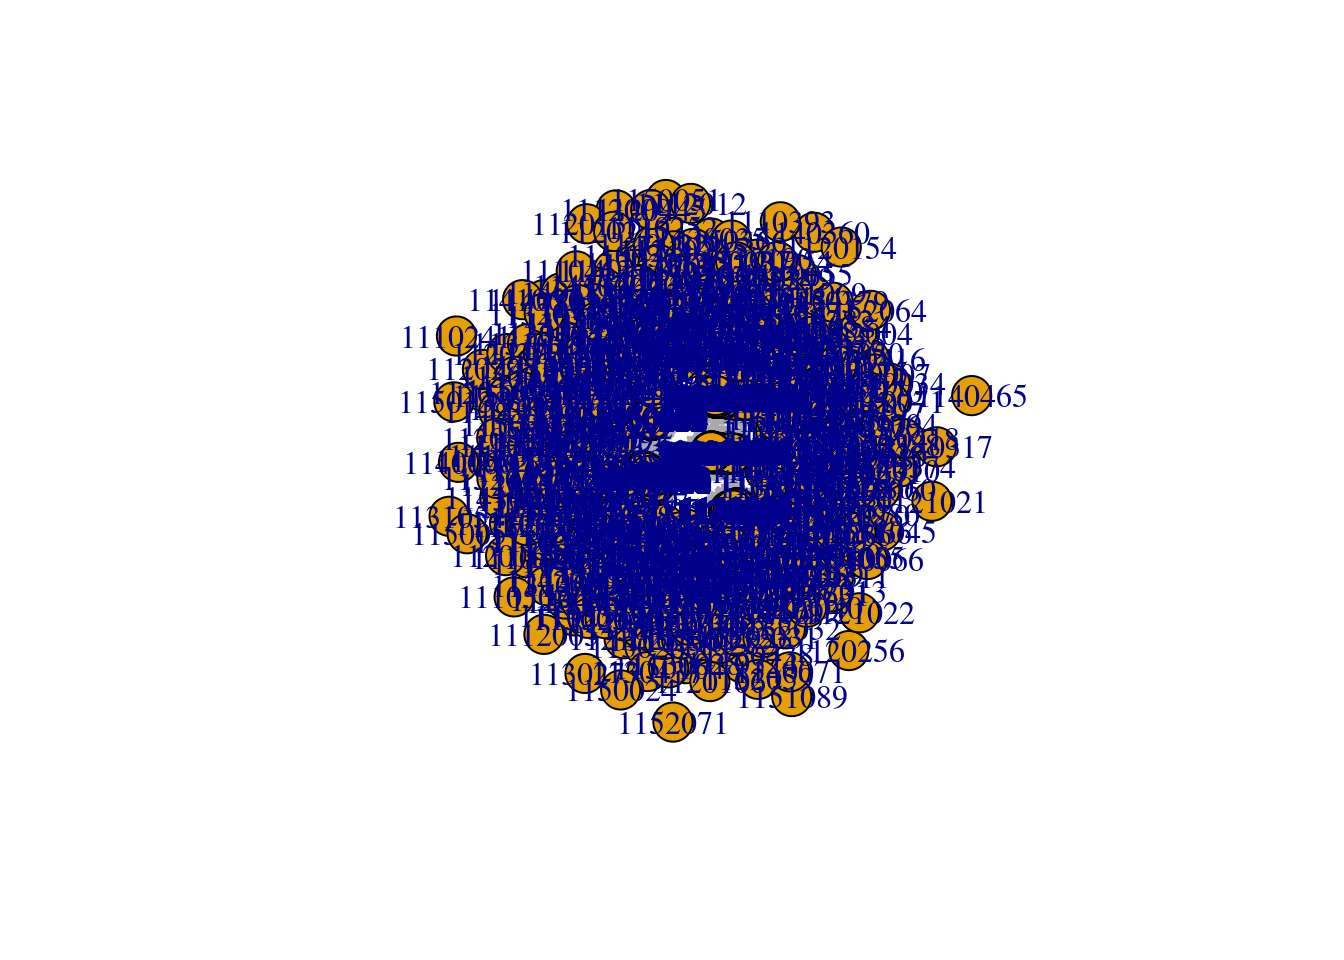
\includegraphics{appliedsnar_files/figure-latex/03-plot-raw-1} 

}

\caption{A not very nice network plot. This is what we get with the default parameters in igraph.}\label{fig:03-plot-raw}
\end{figure}

Not very nice, right? A couple of things with this plot:

\begin{enumerate}
\def\labelenumi{\arabic{enumi}.}
\item
  We are looking at all schools simultaneously, which does not make
  sense. So, instead of plotting \texttt{ig\_year1}, we will focus on
  \texttt{ig\_year1\_111}.
\item
  All the vertices have the same size, and more over, are overalaping.
  So, instead of using the default size, we will size the vertices by
  indegree using the \texttt{degree} function, and passing the vector of
  degrees to \texttt{vertex.size}.\footnote{Figuring out what is the
    optimal vertex size is a bit tricky. Without getting too technical,
    there's no other way of getting \emph{nice} vertex size other than
    just playing with different values of it. A nice solution to this is
    using
    \href{https://www.rdocumentation.org/packages/netdiffuseR/versions/1.17.0/topics/rescale_vertex_igraph}{\texttt{netdiffuseR::igraph\_vertex\_rescale}}
    which rescales the vertices so that these keep their aspect ratio to
    a predefined proportion of the screen.}
\item
  Given the number of vertices in these networks, the labels are not
  useful here. So we will remove them by setting
  \texttt{vertex.label\ =\ NA}. Moreover, we will reduce the size of the
  arrows' tip by setting \texttt{edge.arrow.size\ =\ 0.25}.
\item
  And finally, we will set the color of each vertex to be a function of
  whether the individual is hispanic or not. For this last bit we need
  to go a bit more of programming:
\end{enumerate}

\begin{Shaded}
\begin{Highlighting}[]
\NormalTok{col_hispanic <-}\StringTok{ }\KeywordTok{V}\NormalTok{(ig_year1_}\DecValTok{111}\NormalTok{)}\OperatorTok{$}\NormalTok{hispanic }\OperatorTok{+}\StringTok{ }\DecValTok{1}
\NormalTok{col_hispanic <-}\StringTok{ }\KeywordTok{coalesce}\NormalTok{(col_hispanic, }\DecValTok{3}\NormalTok{) }
\NormalTok{col_hispanic <-}\StringTok{ }\KeywordTok{c}\NormalTok{(}\StringTok{"steelblue"}\NormalTok{, }\StringTok{"tomato"}\NormalTok{, }\StringTok{"white"}\NormalTok{)[col_hispanic]}
\end{Highlighting}
\end{Shaded}

Line by line, we did the following:

\begin{enumerate}
\def\labelenumi{\arabic{enumi}.}
\item
  The first line added one to all no \texttt{NA} values, so that the 0s
  (non-hispanic) turned to 1s and the 1s (hispanic) turned to 2s.
\item
  The second line replaced all \texttt{NA}s with the number 3, so that
  our vector \texttt{col\_hispanic} now ranges from 1 to 3 with no
  \texttt{NA}s in it.
\item
  In the last line we created a vector of colors. Essentially, what we
  are doing here is telling R to create a vector of length
  \texttt{length(col\_hispanic)} by selecting elements by index from the
  vector \texttt{c("steelblue",\ "tomato",\ "white")}. This way, if, for
  example, the first element of the vector \texttt{col\_hispanic} was a
  3, our new vector of colors would have a \texttt{"white"} in it.
\end{enumerate}

To make sure we know we are right, let's print the first 10 elements of
our new vector of colors together with the original \texttt{hispanic}
column:

\begin{Shaded}
\begin{Highlighting}[]
\KeywordTok{cbind}\NormalTok{(}
  \DataTypeTok{original =} \KeywordTok{V}\NormalTok{(ig_year1_}\DecValTok{111}\NormalTok{)}\OperatorTok{$}\NormalTok{hispanic[}\DecValTok{1}\OperatorTok{:}\DecValTok{10}\NormalTok{],}
  \DataTypeTok{colors   =}\NormalTok{ col_hispanic[}\DecValTok{1}\OperatorTok{:}\DecValTok{10}\NormalTok{]}
\NormalTok{  )}
\end{Highlighting}
\end{Shaded}

\begin{verbatim}
##       original colors     
##  [1,] "1"      "tomato"   
##  [2,] "1"      "tomato"   
##  [3,] "0"      "steelblue"
##  [4,] "1"      "tomato"   
##  [5,] "1"      "tomato"   
##  [6,] "1"      "tomato"   
##  [7,] "1"      "tomato"   
##  [8,] "1"      "tomato"   
##  [9,] "0"      "steelblue"
## [10,] "1"      "tomato"
\end{verbatim}

With our nice vector of colors, now we can pass it to
\texttt{plot.igraph} (which we call implicitly by just calling
\texttt{plot}), via the \texttt{vertex.color} argument:

\begin{Shaded}
\begin{Highlighting}[]
\CommentTok{# Fancy graph}
\KeywordTok{set.seed}\NormalTok{(}\DecValTok{1}\NormalTok{)}
\KeywordTok{plot}\NormalTok{(}
\NormalTok{  ig_year1_}\DecValTok{111}\NormalTok{,}
  \DataTypeTok{vertex.size     =} \KeywordTok{degree}\NormalTok{(ig_year1_}\DecValTok{111}\NormalTok{)}\OperatorTok{/}\DecValTok{10} \OperatorTok{+}\DecValTok{1}\NormalTok{,}
  \DataTypeTok{vertex.label    =} \OtherTok{NA}\NormalTok{,}
  \DataTypeTok{edge.arrow.size =}\NormalTok{ .}\DecValTok{25}\NormalTok{,}
  \DataTypeTok{vertex.color    =}\NormalTok{ col_hispanic}
\NormalTok{  )}
\end{Highlighting}
\end{Shaded}

\begin{figure}
\centering
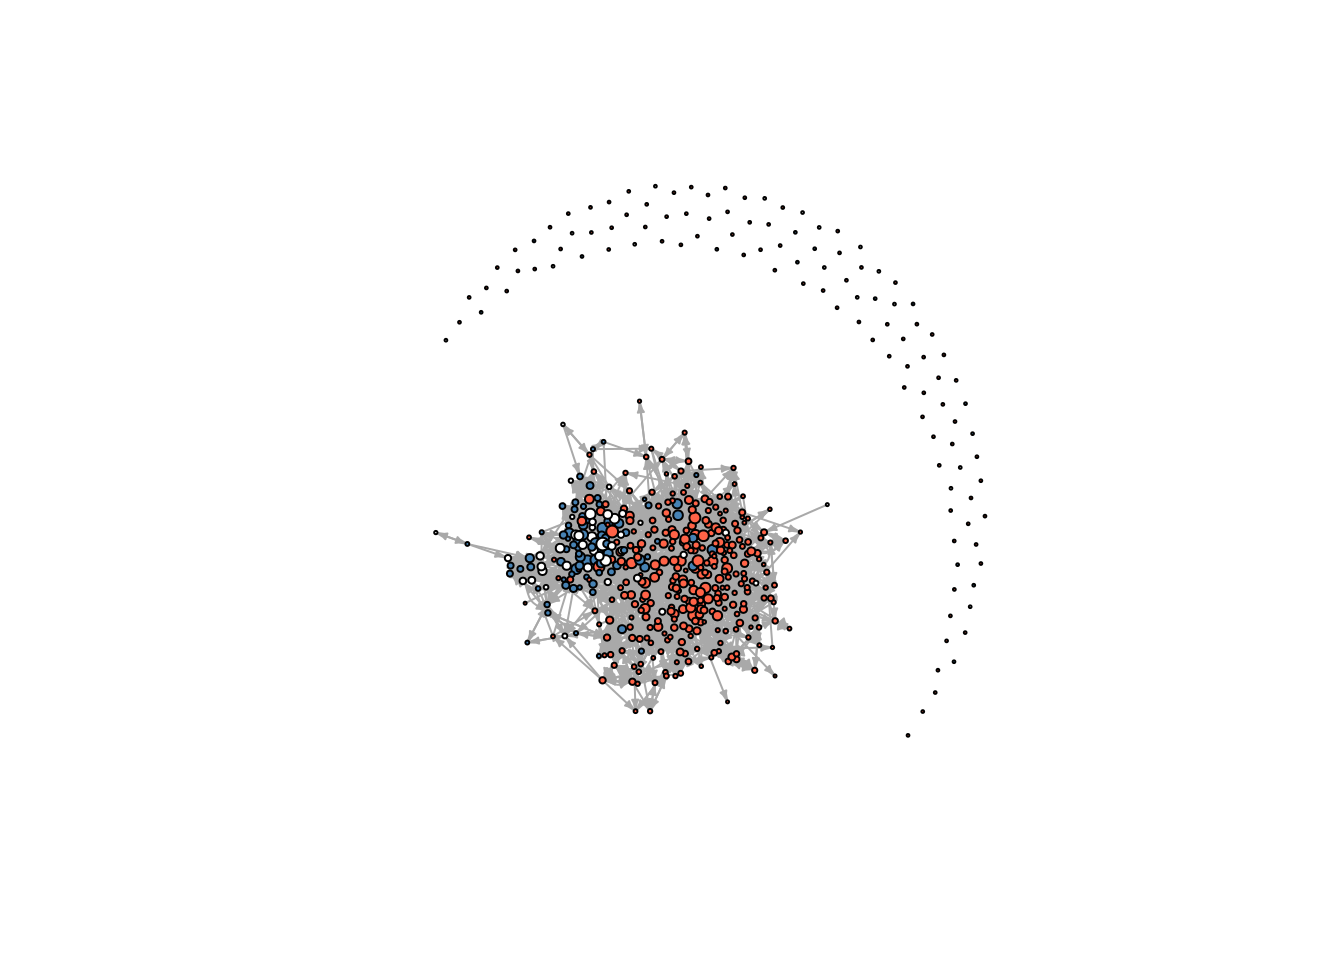
\includegraphics{appliedsnar_files/figure-latex/03-plot-neat1-1.pdf}
\caption{\label{fig:03-plot-neat1}Friends network in time 1 for school 111.}
\end{figure}

Nice! So it does look better. The only problem is that we have a lot of
isolates. Let's try again by drawing the same plot without isolates. To
do so we need to filter the graph, for which we will use the function
\texttt{induced\_subgraph}

\begin{Shaded}
\begin{Highlighting}[]
\CommentTok{# Which vertices are not isolates?}
\NormalTok{which_ids <-}\StringTok{ }\KeywordTok{which}\NormalTok{(}\KeywordTok{degree}\NormalTok{(ig_year1_}\DecValTok{111}\NormalTok{, }\DataTypeTok{mode =} \StringTok{"total"}\NormalTok{) }\OperatorTok{>}\StringTok{ }\DecValTok{0}\NormalTok{)}

\CommentTok{# Getting the subgraph}
\NormalTok{ig_year1_111_sub <-}\StringTok{ }\KeywordTok{induced_subgraph}\NormalTok{(ig_year1_}\DecValTok{111}\NormalTok{, which_ids)}

\CommentTok{# We need to get the same subset in col_hispanic}
\NormalTok{col_hispanic <-}\StringTok{ }\NormalTok{col_hispanic[which_ids]}
\end{Highlighting}
\end{Shaded}

\begin{Shaded}
\begin{Highlighting}[]
\CommentTok{# Fancy graph}
\KeywordTok{set.seed}\NormalTok{(}\DecValTok{1}\NormalTok{)}
\KeywordTok{plot}\NormalTok{(}
\NormalTok{  ig_year1_111_sub,}
  \DataTypeTok{vertex.size     =} \KeywordTok{degree}\NormalTok{(ig_year1_111_sub)}\OperatorTok{/}\DecValTok{5} \OperatorTok{+}\DecValTok{1}\NormalTok{,}
  \DataTypeTok{vertex.label    =} \OtherTok{NA}\NormalTok{,}
  \DataTypeTok{edge.arrow.size =}\NormalTok{ .}\DecValTok{25}\NormalTok{,}
  \DataTypeTok{vertex.color    =}\NormalTok{ col_hispanic}
\NormalTok{  )}
\end{Highlighting}
\end{Shaded}

\begin{figure}
\centering
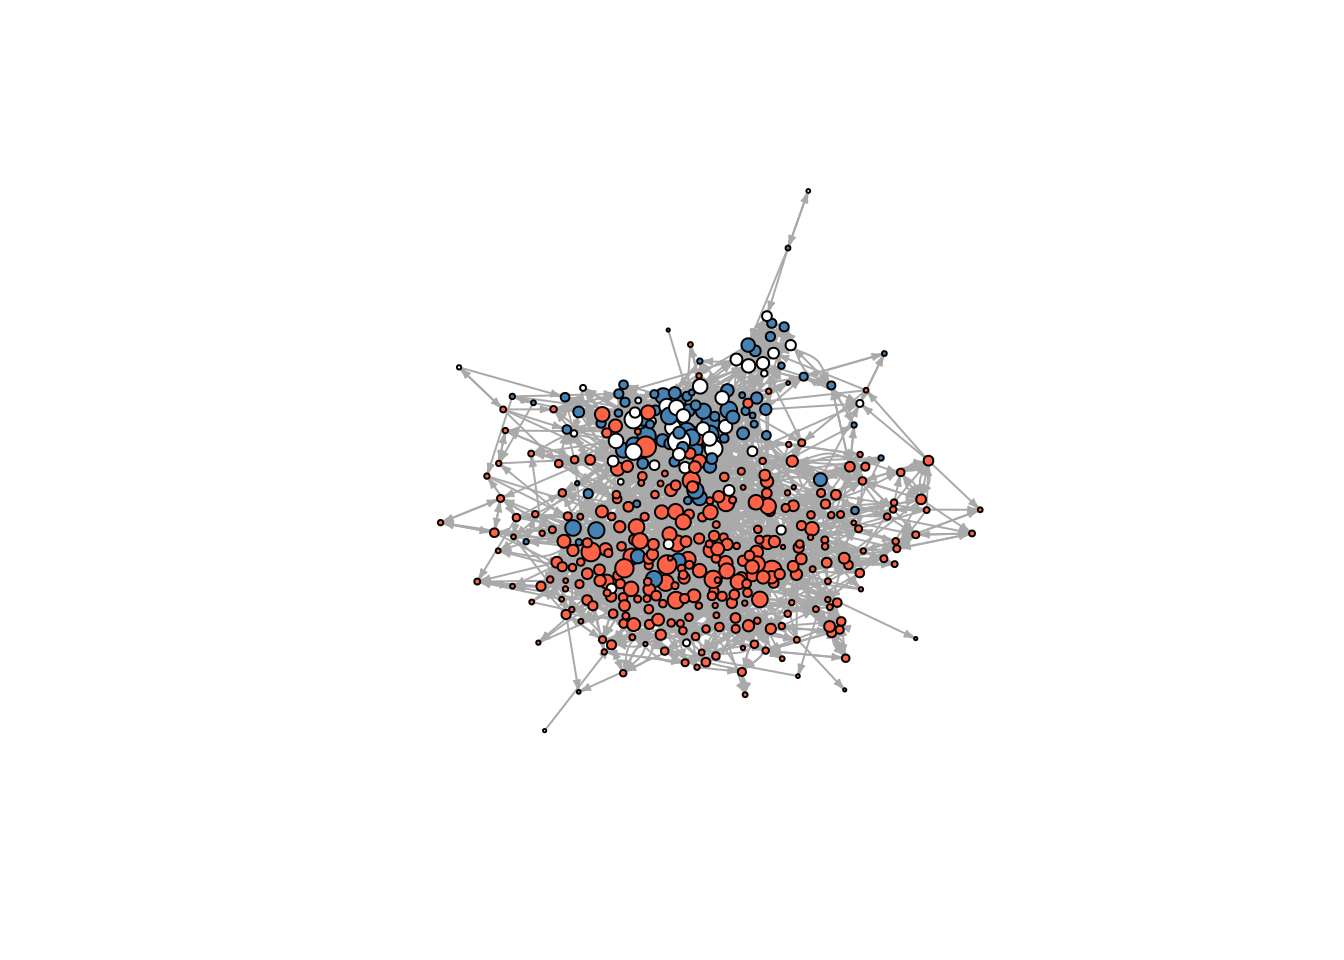
\includegraphics{appliedsnar_files/figure-latex/03-plot-neat2-1.pdf}
\caption{\label{fig:03-plot-neat2}Friends network in time 1 for school 111.
The graph excludes isolates.}
\end{figure}

Now that's better! An interesting pattern that shows up is that
individuals seem to cluster by whether they are hispanic or not.

We can actually write this as a function so that, instead of us copying
and pasting the code \(n\) times (supposing that we want to crate a plot
similar to this \(n\) times). The next subsection does that.

\subsection{Multiple plots}\label{multiple-plots}

When you are repeating yourself over and over again, it is a good idea
to write down a sequence of commands as a function. In this case, since
we will be running the same type of plot for all schools/waves, we write
a function in which the only things that changes are: (a) the school id,
and (b) the color of the nodes.

\begin{Shaded}
\begin{Highlighting}[]
\NormalTok{myplot <-}\StringTok{ }\ControlFlowTok{function}\NormalTok{(}
\NormalTok{  net,}
\NormalTok{  schoolid,}
  \DataTypeTok{mindgr =} \DecValTok{1}\NormalTok{,}
  \DataTypeTok{vcol   =} \StringTok{"tomato"}\NormalTok{,}
\NormalTok{  ...) \{}
  
  \CommentTok{# Creating a subgraph}
\NormalTok{  subnet <-}\StringTok{ }\KeywordTok{induced_subgraph}\NormalTok{(}
\NormalTok{    net,}
    \KeywordTok{which}\NormalTok{(}\KeywordTok{degree}\NormalTok{(net, }\DataTypeTok{mode =} \StringTok{"all"}\NormalTok{) }\OperatorTok{>=}\StringTok{ }\NormalTok{mindgr }\OperatorTok{&}\StringTok{ }\KeywordTok{V}\NormalTok{(net)}\OperatorTok{$}\NormalTok{school }\OperatorTok{==}\StringTok{ }\NormalTok{schoolid)}
\NormalTok{  )}
  
  \CommentTok{# Fancy graph}
  \KeywordTok{set.seed}\NormalTok{(}\DecValTok{1}\NormalTok{)}
  \KeywordTok{plot}\NormalTok{(}
\NormalTok{    subnet,}
    \DataTypeTok{vertex.size     =} \KeywordTok{degree}\NormalTok{(subnet)}\OperatorTok{/}\DecValTok{5}\NormalTok{,}
    \DataTypeTok{vertex.label    =} \OtherTok{NA}\NormalTok{,}
    \DataTypeTok{edge.arrow.size =}\NormalTok{ .}\DecValTok{25}\NormalTok{,}
    \DataTypeTok{vertex.color    =}\NormalTok{ vcol,}
\NormalTok{    ...}
\NormalTok{    )}
\NormalTok{\}}
\end{Highlighting}
\end{Shaded}

The function definition:

\begin{enumerate}
\def\labelenumi{\arabic{enumi}.}
\item
  The
  \texttt{myplot\ \textless{}-\ function({[}arguments{]})\ \{{[}body\ of\ the\ function{]}\}}
  tells R that we are going to create a function called \texttt{myplot}.
\item
  In the arguments part, we are declaring 4 specific arguments:
  \texttt{net}, \texttt{schoolid}, \texttt{mindgr}, and \texttt{vcol}.
  These are an igraph object, the school id, the minimum degree that a
  vertex must have to be included in the plot, and the color of the
  vertices. Notice that, as a difference from other programming
  languages, in R we don't need to declare the types that these objects
  are.
\item
  The elipsis object, \texttt{...}, is a special object in R that allows
  us passing other arguments without us specifying which. In our case,
  if you take a look at the \texttt{plot} bit of the body of the
  function, you will see that we also added \texttt{...}; this means
  that whatever other arguments (different from the ones that we
  explicitly defined) are passed to the function, these will be passed
  to the function \texttt{plot}, moreover, to the \texttt{plot.gexf}
  function (since the \texttt{subnet} object is actually an igraph
  object). In practice, this implies that we can, for example, set the
  argument \texttt{edge.arrow.size} when calling \texttt{myplot}, even
  though we did not included it in the function definition! (See
  \texttt{?dotsMethods} in R for more details).
\end{enumerate}

In the following lines of code, using our new function, we will plot
each schools' network in the same plotting device (window) with the help
of the \texttt{par} function, and add legend with the \texttt{legend}:

\begin{Shaded}
\begin{Highlighting}[]
\CommentTok{# Plotting all together}
\NormalTok{oldpar <-}\StringTok{ }\KeywordTok{par}\NormalTok{(}\DataTypeTok{no.readonly =} \OtherTok{TRUE}\NormalTok{)}
\KeywordTok{par}\NormalTok{(}\DataTypeTok{mfrow =} \KeywordTok{c}\NormalTok{(}\DecValTok{2}\NormalTok{, }\DecValTok{3}\NormalTok{), }\DataTypeTok{mai =} \KeywordTok{rep}\NormalTok{(}\DecValTok{0}\NormalTok{, }\DecValTok{4}\NormalTok{), }\DataTypeTok{oma=} \KeywordTok{c}\NormalTok{(}\DecValTok{1}\NormalTok{, }\DecValTok{0}\NormalTok{, }\DecValTok{0}\NormalTok{, }\DecValTok{0}\NormalTok{))}
\KeywordTok{myplot}\NormalTok{(ig_year1, }\DecValTok{111}\NormalTok{, }\DataTypeTok{vcol =} \StringTok{"tomato"}\NormalTok{)}
\KeywordTok{myplot}\NormalTok{(ig_year1, }\DecValTok{112}\NormalTok{, }\DataTypeTok{vcol =} \StringTok{"steelblue"}\NormalTok{)}
\KeywordTok{myplot}\NormalTok{(ig_year1, }\DecValTok{113}\NormalTok{, }\DataTypeTok{vcol =} \StringTok{"black"}\NormalTok{)}
\KeywordTok{myplot}\NormalTok{(ig_year1, }\DecValTok{114}\NormalTok{, }\DataTypeTok{vcol =} \StringTok{"gold"}\NormalTok{)}
\KeywordTok{myplot}\NormalTok{(ig_year1, }\DecValTok{115}\NormalTok{, }\DataTypeTok{vcol =} \StringTok{"white"}\NormalTok{)}
\KeywordTok{par}\NormalTok{(oldpar)}

\CommentTok{# A fancy legend}
\KeywordTok{legend}\NormalTok{(}
  \StringTok{"bottomright"}\NormalTok{,}
  \DataTypeTok{legend =} \KeywordTok{c}\NormalTok{(}\DecValTok{111}\NormalTok{, }\DecValTok{112}\NormalTok{, }\DecValTok{113}\NormalTok{, }\DecValTok{114}\NormalTok{, }\DecValTok{115}\NormalTok{),}
  \DataTypeTok{pt.bg  =} \KeywordTok{c}\NormalTok{(}\StringTok{"tomato"}\NormalTok{, }\StringTok{"steelblue"}\NormalTok{, }\StringTok{"black"}\NormalTok{, }\StringTok{"gold"}\NormalTok{, }\StringTok{"white"}\NormalTok{),}
  \DataTypeTok{pch    =} \DecValTok{21}\NormalTok{,}
  \DataTypeTok{cex    =} \DecValTok{1}\NormalTok{,}
  \DataTypeTok{bty    =} \StringTok{"n"}\NormalTok{,}
  \DataTypeTok{title  =} \StringTok{"School"}
\NormalTok{  )}
\end{Highlighting}
\end{Shaded}

\begin{figure}
\centering
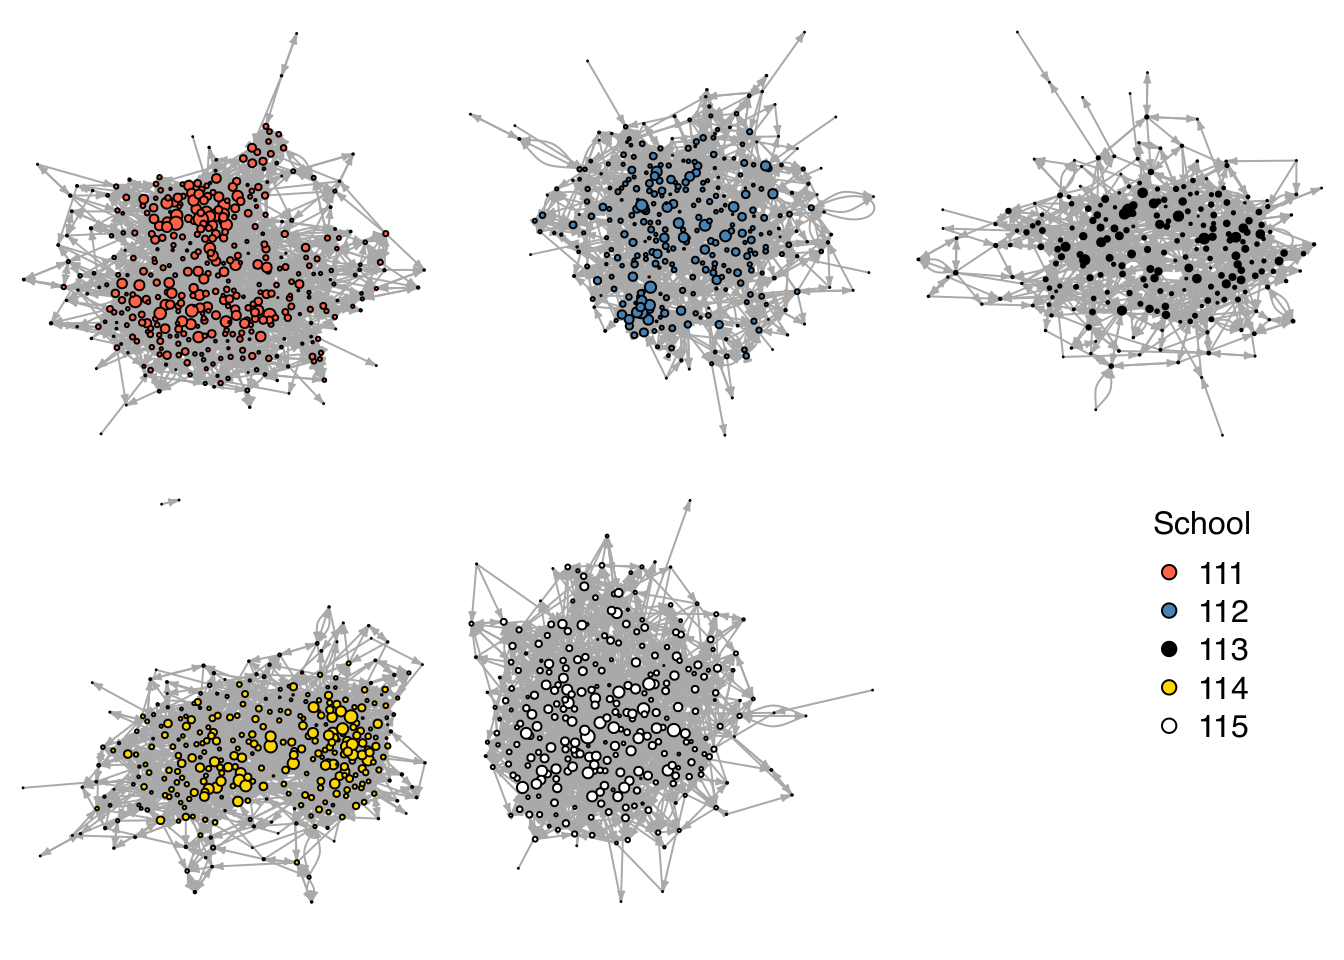
\includegraphics{appliedsnar_files/figure-latex/03-myplot-call-1.pdf}
\caption{\label{fig:03-myplot-call}All 5 schools in time 1. Again, the
graphs exclude isolates.}
\end{figure}

So what happend here?

\begin{itemize}
\item
  \texttt{oldpar\ \textless{}-\ par(no.readonly\ =\ TRUE)} This line
  stores the current parameters for plotting. Since we are going to be
  changing them, we better make sure we are able to go back!.
\item
  \texttt{par(mfrow\ =\ c(2,\ 3),\ mai\ =\ rep(0,\ 4),\ oma=rep(0,\ 4))}
  Here we are setting various things at the same time. \texttt{mfrow}
  specifies how many \emph{figures} will be drawn and in what order, in
  particular, we are asking the plotting device to allow for 2*3 = 6
  plots organized in 2 rows and 3 columns, and these will be drawn by
  row.

  \texttt{mai} specifies the size of the margins in inches. Setting all
  margins equal to zero (which is what we are doing now) gives more
  space to the network itself. The same is true for \texttt{oma}. See
  \texttt{?par} for more info.
\item
  \texttt{myplot(ig\_year1,\ ...)} This is simply calling our plotting
  function. The neat part of this is that, since we set
  \texttt{mfrow\ =\ c(2,\ 3)}, R takes care of \emph{distributing} the
  plots in the device.
\item
  \texttt{par(oldpar)} This line allows us to restore the plotting
  parameters.
\end{itemize}

\section{Statistical tests}\label{statistical-tests}

\subsection{Is nomination number correlated with
indegree?}\label{is-nomination-number-correlated-with-indegree}

Hypothesis: Individuals that on average are among the first nominations
of their peers are more popular

\begin{Shaded}
\begin{Highlighting}[]
\CommentTok{# Getting all the data in long format}
\NormalTok{edgelist <-}\StringTok{ }\KeywordTok{as_long_data_frame}\NormalTok{(ig_year1) }\OperatorTok
\StringTok{  }\NormalTok{as_tibble}

\CommentTok{# Computing indegree (again) and average nomination number}
\CommentTok{# Include "On a scale from one to five how close do you feel"}
\CommentTok{# Also for egocentric friends (A. Friends)}
\NormalTok{indeg_nom_cor <-}\StringTok{ }\KeywordTok{group_by}\NormalTok{(edgelist, to, to_name, to_school) }\OperatorTok
\StringTok{  }\KeywordTok{summarise}\NormalTok{(}
    \DataTypeTok{indeg   =} \KeywordTok{n}\NormalTok{(),}
    \DataTypeTok{nom_avg =} \DecValTok{1}\OperatorTok{/}\KeywordTok{mean}\NormalTok{(nnom)}
\NormalTok{  ) }\OperatorTok
\StringTok{  }\KeywordTok{rename}\NormalTok{(}
    \DataTypeTok{school =}\NormalTok{ to_school}
\NormalTok{  )}

\NormalTok{indeg_nom_cor}
\end{Highlighting}
\end{Shaded}

\begin{verbatim}
## # A tibble: 1,561 x 5
## # Groups:   to, to_name [1,561]
##       to to_name school indeg nom_avg
##    <dbl> <chr>    <int> <int>   <dbl>
##  1    2. 1110002    111    22   0.222
##  2    3. 1110007    111     7   0.175
##  3    4. 1110013    111     6   0.171
##  4    5. 1110014    111    19   0.134
##  5    6. 1110015    111     3   0.150
##  6    7. 1110020    111     6   0.154
##  7    9. 1110025    111     6   0.214
##  8   10. 1110027    111    13   0.220
##  9   11. 1110029    111    14   0.131
## 10   12. 1110030    111     6   0.222
## # ... with 1,551 more rows
\end{verbatim}

\begin{Shaded}
\begin{Highlighting}[]
\CommentTok{# Using pearson's correlation}
\KeywordTok{with}\NormalTok{(indeg_nom_cor, }\KeywordTok{cor.test}\NormalTok{(indeg, nom_avg))}
\end{Highlighting}
\end{Shaded}

\begin{verbatim}
## 
##  Pearson's product-moment correlation
## 
## data:  indeg and nom_avg
## t = -12.254, df = 1559, p-value < 2.2e-16
## alternative hypothesis: true correlation is not equal to 0
## 95 percent confidence interval:
##  -0.3409964 -0.2504653
## sample estimates:
##        cor 
## -0.2963965
\end{verbatim}

\begin{Shaded}
\begin{Highlighting}[]
\KeywordTok{save.image}\NormalTok{(}\StringTok{"03.rda"}\NormalTok{)}
\end{Highlighting}
\end{Shaded}

\chapter{SNS Exponential Random Graph
Models}\label{sns-exponential-random-graph-models}

I strongly suggest reading the vignette included in the \texttt{ergm} R
package

\begin{Shaded}
\begin{Highlighting}[]
\KeywordTok{vignette}\NormalTok{(}\StringTok{"ergm"}\NormalTok{, }\DataTypeTok{package=}\StringTok{"ergm"}\NormalTok{)}
\end{Highlighting}
\end{Shaded}

So what are ERGMs anyway\ldots{}

\begin{quote}
The purpose of ERGMs, in a nutshell, is to describe parsimoniously the
local selection forces that shape the global structure of a network. To
this end, a network dataset, like those depicted in Figure 1, may be
considered like the response in a regression model, where the predictors
are things like ``propensity for individuals of the same sex to form
partnerships'' or ``propensity for individuals to form triangles of
partnerships''. In Figure 1(b), for example, it is evident that the
individual nodes appear to cluster in groups of the same numerical
labels (which turn out to be students' grades, 7 through 12); thus, an
ERGM can help us quantify the strength of this intra-group effect.

--- (Hunter et al. \protect\hyperlink{ref-Hunter2008}{2008})
\end{quote}

\begin{figure}
\centering
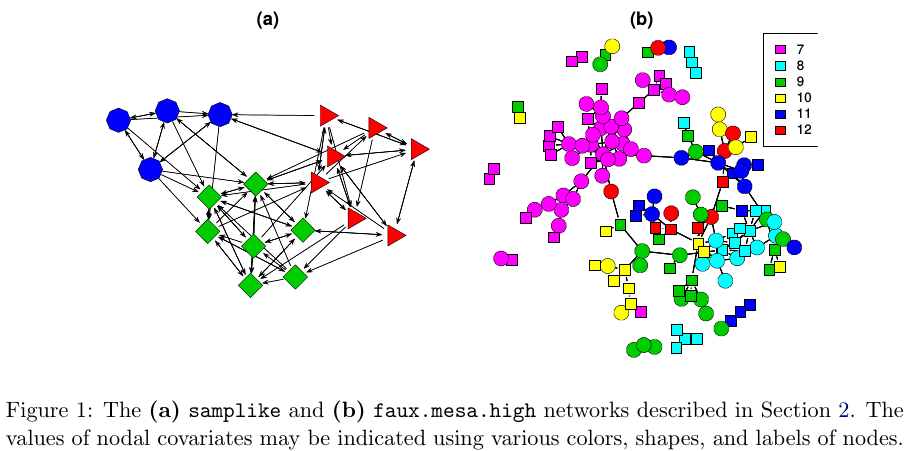
\includegraphics{hunter2008.png}
\caption{Source: Hunter et al. (2008)}
\end{figure}

The distribution of \(\mathbf{Y}\) can be parameterized in the form

\[
\Pr{\mathbf{Y}=\mathbf{y}|\theta, \mathcal{Y}} = \frac{\exp{\theta^{\mbox{T}}\mathbf{g}(\mathbf{y})}}{\kappa\left(\theta, \mathcal{Y}\right)},\quad\mathbf{y}\in\mathcal{Y}
\label{eq:04-1}
\]

Where \(\theta\in\Omega\subset\mathbb{R}^q\) is the vector of model
coefficients and \(\mathbf{g}(\mathbf{y})\) is a \emph{q}-vector of
statistics based on the adjacency matrix \(\mathbf{y}\).

Model \eqref{eq:04-1} may be expanded by replacing
\(\mathbf{g}(\mathbf{y})\) with \(\mathbf{g}(\mathbf{y}, \mathbf{X})\)
to allow for additional covariate information \(\mathbf{X}\) about the
network. The denominator,

\[
\kappa\left(\theta,\mathcal{Y}\right) = \sum_{\mathbf{z}\in\mathcal{Y}}\exp{\theta^{\mbox{T}}\mathbf{g}(\mathbf{z})}
\]

Is the normalizing factor that ensures that equation \eqref{eq:04-1} is a
legitimate probability distribution. Even after fixing \(\mathcal{Y}\)
to be all the networks that have size \(n\), the size of \(\mathcal{Y}\)
makes this type of models hard to estimate as there are
\(N = 2^{n(n-1)}\) possible networks! (Hunter et al.
\protect\hyperlink{ref-Hunter2008}{2008})

\section{\texorpdfstring{The \texttt{ergm}
package}{The ergm package}}\label{the-ergm-package}

The \texttt{ergm} R package (Handcock et al.
\protect\hyperlink{ref-R-ergm}{2017})

From the previous section:\footnote{You can download the 03.rda file
  from \href{https://github.com/gvegayon/appliedsnar}{this link}.}

\begin{Shaded}
\begin{Highlighting}[]
\KeywordTok{library}\NormalTok{(igraph)}
\KeywordTok{library}\NormalTok{(magrittr)}
\KeywordTok{library}\NormalTok{(dplyr)}

\KeywordTok{load}\NormalTok{(}\StringTok{"03.rda"}\NormalTok{)}
\end{Highlighting}
\end{Shaded}

In this section we will use the \texttt{ergm} package (from the
\texttt{statnet} suit of packages (Handcock et al.
\protect\hyperlink{ref-R-statnet}{2016})) suit, and the
\texttt{intergraph} (Bojanowski
\protect\hyperlink{ref-R-intergraph}{2015}) package. The latter provides
functions to go back and forth between \texttt{igraph} and
\texttt{network} objects from the \texttt{igraph} and \texttt{network}
packages respectively\footnote{Yes, the classes have the same name as
  the packages.}

\begin{Shaded}
\begin{Highlighting}[]
\KeywordTok{library}\NormalTok{(ergm)}
\KeywordTok{library}\NormalTok{(intergraph)}
\end{Highlighting}
\end{Shaded}

As a rather important side note, the order in which R packages are
loaded matters. Why is this important to mention now? Well, it turns out
that at least a couple of functions in the \texttt{network} package have
the same name of some functions in the \texttt{igraph} package. When the
\texttt{ergm} package is loaded, since it depends on \texttt{network},
it will load the \texttt{network} package first, which will \emph{mask}
some functions in \texttt{igraph}. This becomes evident once you load
\texttt{ergm} after loading \texttt{igraph}:

\begin{verbatim}
The following objects are masked from ‘package:igraph’:

  add.edges, add.vertices, %c%, delete.edges, delete.vertices, get.edge.attribute, get.edges,
  get.vertex.attribute, is.bipartite, is.directed, list.edge.attributes, list.vertex.attributes, %s%,
  set.edge.attribute, set.vertex.attribute
\end{verbatim}

What are the implications of this? If you call the function
\texttt{list.edge.attributes} for an object of class \texttt{igraph} R
will return an error as the first function that matches that name comes
from the \texttt{network} package! To avoid this you can use the double
colon notation:

\begin{Shaded}
\begin{Highlighting}[]
\NormalTok{igraph}\OperatorTok{::}\KeywordTok{list.edge.attributes}\NormalTok{(my_igraph_object)}
\NormalTok{network}\OperatorTok{::}\KeywordTok{list.edge.attributes}\NormalTok{(my_network_object)}
\end{Highlighting}
\end{Shaded}

Anyway\ldots{} Using the \texttt{asNetwork} function, we can coerce the
igraph object into a network object so we can use it with the
\texttt{ergm} function:

\begin{Shaded}
\begin{Highlighting}[]
\CommentTok{# Creating the new network}
\NormalTok{network_}\DecValTok{111}\NormalTok{ <-}\StringTok{ }\NormalTok{intergraph}\OperatorTok{::}\KeywordTok{asNetwork}\NormalTok{(ig_year1_}\DecValTok{111}\NormalTok{)}

\CommentTok{# Running a simple ergm (only fitting edge count)}
\KeywordTok{ergm}\NormalTok{(network_}\DecValTok{111} \OperatorTok{~}\StringTok{ }\NormalTok{edges)}
\end{Highlighting}
\end{Shaded}

\begin{verbatim}
## [1] "Warning:  This network contains loops"
## [1] "Warning:  This network contains loops"
## [1] "Warning:  This network contains loops"
\end{verbatim}

\begin{verbatim}
## Evaluating log-likelihood at the estimate.
\end{verbatim}

\begin{verbatim}
## 
## MLE Coefficients:
##  edges  
## -4.732
\end{verbatim}

So what happened here! We got a warning. It turns out that our network
has loops (didn't thought about it before!). Let's take a look on that
with the \texttt{which\_loop} function

\begin{Shaded}
\begin{Highlighting}[]
\KeywordTok{E}\NormalTok{(ig_year1_}\DecValTok{111}\NormalTok{)[}\KeywordTok{which_loop}\NormalTok{(ig_year1_}\DecValTok{111}\NormalTok{)]}
\end{Highlighting}
\end{Shaded}

\begin{verbatim}
## + 1/2638 edge from 76b6f3b (vertex names):
## [1] 1110111->1110111
\end{verbatim}

We can get rid of these using the \texttt{igraph::-.igraph}. Moreover,
just to illustrate how it can be done, let's get rid of the isolates
using the same operator

\begin{Shaded}
\begin{Highlighting}[]
\CommentTok{# Creating the new network}
\NormalTok{network_}\DecValTok{111}\NormalTok{ <-}\StringTok{ }\NormalTok{ig_year1_}\DecValTok{111}

\CommentTok{# Removing loops}
\NormalTok{network_}\DecValTok{111}\NormalTok{ <-}\StringTok{ }\NormalTok{network_}\DecValTok{111} \OperatorTok{-}\StringTok{ }\KeywordTok{E}\NormalTok{(network_}\DecValTok{111}\NormalTok{)[}\KeywordTok{which}\NormalTok{(}\KeywordTok{which_loop}\NormalTok{(network_}\DecValTok{111}\NormalTok{))]}

\CommentTok{# Removing isolates}
\NormalTok{network_}\DecValTok{111}\NormalTok{ <-}\StringTok{ }\NormalTok{network_}\DecValTok{111} \OperatorTok{-}\StringTok{ }\KeywordTok{which}\NormalTok{(}\KeywordTok{degree}\NormalTok{(network_}\DecValTok{111}\NormalTok{, }\DataTypeTok{mode =} \StringTok{"all"}\NormalTok{) }\OperatorTok{==}\StringTok{ }\DecValTok{0}\NormalTok{)}

\CommentTok{# Converting the network}
\NormalTok{network_}\DecValTok{111}\NormalTok{ <-}\StringTok{ }\NormalTok{intergraph}\OperatorTok{::}\KeywordTok{asNetwork}\NormalTok{(network_}\DecValTok{111}\NormalTok{)}
\end{Highlighting}
\end{Shaded}

\section{Running ERGMs}\label{running-ergms}

Proposed workflow:

\begin{enumerate}
\def\labelenumi{\arabic{enumi}.}
\item
  Estimate the simplest model, adding one variable at a time.
\item
  After each estimation, run the \texttt{mcmc.diagnostics} function to
  see how good/bad behaved are the chains.
\item
  Run the \texttt{gof} function to see how good is the model at matching
  the network's structural statistics.
\end{enumerate}

What to use:

\begin{enumerate}
\def\labelenumi{\arabic{enumi}.}
\item
  \texttt{control.ergms}: Maximum number of iteration, seed for
  Pseudo-RNG, how many cores
\item
  \texttt{ergm.constraints}: Where to sample the network from. Gives
  stability and (in some cases) faster convergence as by constraining
  the model you are reducing the sample size.
\end{enumerate}

Here is an example of a couple of models that we could compare\footnote{Notice
  that this document may not include the usual messages that the
  \texttt{ergm} command generates during the estimation procedure. This
  is just to make it more printable-friendly.}

\begin{Shaded}
\begin{Highlighting}[]
\NormalTok{ans0 <-}\StringTok{ }\KeywordTok{ergm}\NormalTok{(}
\NormalTok{  network_}\DecValTok{111} \OperatorTok{~}
\StringTok{    }\NormalTok{edges }\OperatorTok{+}
\StringTok{    }\KeywordTok{nodematch}\NormalTok{(}\StringTok{"hispanic"}\NormalTok{) }\OperatorTok{+}
\StringTok{    }\KeywordTok{nodematch}\NormalTok{(}\StringTok{"female1"}\NormalTok{) }\OperatorTok{+}
\StringTok{    }\KeywordTok{nodematch}\NormalTok{(}\StringTok{"eversmk1"}\NormalTok{) }\OperatorTok{+}
\StringTok{    }\NormalTok{mutual}
\NormalTok{    ,}
  \DataTypeTok{constraints =} \OperatorTok{~}\KeywordTok{bd}\NormalTok{(}\DataTypeTok{maxout =} \DecValTok{19}\NormalTok{),}
  \DataTypeTok{control =} \KeywordTok{control.ergm}\NormalTok{(}
    \DataTypeTok{seed        =} \DecValTok{1}\NormalTok{,}
    \DataTypeTok{MCMLE.maxit =} \DecValTok{10}\NormalTok{,}
    \DataTypeTok{parallel    =} \DecValTok{4}\NormalTok{,}
    \DataTypeTok{CD.maxit    =} \DecValTok{10}
\NormalTok{    )}
\NormalTok{  )}
\end{Highlighting}
\end{Shaded}

So what are we doing here: 1. The model is controling for: a.
\texttt{edges} Number of edges in the network (as opposed to its
density) b. \texttt{nodematch("some-variable-name-here")} Includes a
term that controls for homophily/heterophily c. \texttt{mutual} Number
of mutual connections between \(i\) and \(j\). This can be related to,
for example, triadic closure.

\begin{Shaded}
\begin{Highlighting}[]
\NormalTok{ans1 <-}\StringTok{ }\KeywordTok{ergm}\NormalTok{(}
\NormalTok{  network_}\DecValTok{111} \OperatorTok{~}
\StringTok{    }\NormalTok{edges }\OperatorTok{+}
\StringTok{    }\KeywordTok{nodematch}\NormalTok{(}\StringTok{"hispanic"}\NormalTok{) }\OperatorTok{+}
\StringTok{    }\KeywordTok{nodematch}\NormalTok{(}\StringTok{"female1"}\NormalTok{) }\OperatorTok{+}
\StringTok{    }\KeywordTok{nodematch}\NormalTok{(}\StringTok{"eversmk1"}\NormalTok{)}
\NormalTok{    ,}
  \DataTypeTok{constraints =} \OperatorTok{~}\KeywordTok{bd}\NormalTok{(}\DataTypeTok{maxout =} \DecValTok{19}\NormalTok{),}
  \DataTypeTok{control =} \KeywordTok{control.ergm}\NormalTok{(}
    \DataTypeTok{seed        =} \DecValTok{1}\NormalTok{,}
    \DataTypeTok{MCMLE.maxit =} \DecValTok{10}\NormalTok{,}
    \DataTypeTok{parallel    =} \DecValTok{4}\NormalTok{,}
    \DataTypeTok{CD.maxit    =} \DecValTok{10}
\NormalTok{    )}
\NormalTok{  )}
\end{Highlighting}
\end{Shaded}

This example takes longer to compute

\begin{Shaded}
\begin{Highlighting}[]
\NormalTok{ans2 <-}\StringTok{ }\KeywordTok{ergm}\NormalTok{(}
\NormalTok{  network_}\DecValTok{111} \OperatorTok{~}
\StringTok{    }\NormalTok{edges }\OperatorTok{+}
\StringTok{    }\KeywordTok{nodematch}\NormalTok{(}\StringTok{"hispanic"}\NormalTok{) }\OperatorTok{+}
\StringTok{    }\KeywordTok{nodematch}\NormalTok{(}\StringTok{"female1"}\NormalTok{) }\OperatorTok{+}
\StringTok{    }\KeywordTok{nodematch}\NormalTok{(}\StringTok{"eversmk1"}\NormalTok{) }\OperatorTok{+}\StringTok{ }
\StringTok{    }\NormalTok{mutual }\OperatorTok{+}
\StringTok{    }\NormalTok{balance}
\NormalTok{    ,}
  \DataTypeTok{constraints =} \OperatorTok{~}\KeywordTok{bd}\NormalTok{(}\DataTypeTok{maxout =} \DecValTok{19}\NormalTok{),}
  \DataTypeTok{control =} \KeywordTok{control.ergm}\NormalTok{(}
    \DataTypeTok{seed        =} \DecValTok{1}\NormalTok{,}
    \DataTypeTok{MCMLE.maxit =} \DecValTok{10}\NormalTok{,}
    \DataTypeTok{parallel    =} \DecValTok{4}\NormalTok{,}
    \DataTypeTok{CD.maxit    =} \DecValTok{10}
\NormalTok{    )}
\NormalTok{  )}
\end{Highlighting}
\end{Shaded}

Now, a nice trick to see all regressions in the same table, we can use
the \texttt{texreg} package (Leifeld
\protect\hyperlink{ref-R-texreg}{2013}) which supports \texttt{ergm}
ouputs!

\begin{Shaded}
\begin{Highlighting}[]
\KeywordTok{library}\NormalTok{(texreg)}
\end{Highlighting}
\end{Shaded}

\begin{verbatim}
## Version:  1.36.23
## Date:     2017-03-03
## Author:   Philip Leifeld (University of Glasgow)
## 
## Please cite the JSS article in your publications -- see citation("texreg").
\end{verbatim}

\begin{verbatim}
## 
## Attaching package: 'texreg'
\end{verbatim}

\begin{verbatim}
## The following object is masked from 'package:magrittr':
## 
##     extract
\end{verbatim}

\begin{Shaded}
\begin{Highlighting}[]
\KeywordTok{screenreg}\NormalTok{(}\KeywordTok{list}\NormalTok{(ans0, ans1, ans2))}
\end{Highlighting}
\end{Shaded}

\begin{verbatim}
## Note: The constraint on the sample space is not dyad-independent. Null model likelihood is only implemented for dyad-independent constraints at this time. Number of observations is similarly ill-defined.
\end{verbatim}

\begin{verbatim}
## Note: The constraint on the sample space is not dyad-independent. Null model likelihood is only implemented for dyad-independent constraints at this time. Number of observations is similarly ill-defined.
## Note: The constraint on the sample space is not dyad-independent. Null model likelihood is only implemented for dyad-independent constraints at this time. Number of observations is similarly ill-defined.
\end{verbatim}

\begin{verbatim}
## 
## ===============================================================
##                     Model 1        Model 2        Model 3      
## ---------------------------------------------------------------
## edges                   -5.63 ***      -5.53 ***      -5.56 ***
##                         (0.06)         (0.06)         (0.05)   
## nodematch.hispanic       0.37 ***       0.51 ***       0.38 ***
##                         (0.04)         (0.04)         (0.04)   
## nodematch.female1        0.82 ***       1.10 ***       0.83 ***
##                         (0.04)         (0.05)         (0.04)   
## nodematch.eversmk1       0.33 ***       0.47 ***       0.35 ***
##                         (0.04)         (0.04)         (0.04)   
## mutual                   4.09 ***                     -4.76 ***
##                         (0.07)                        (0.25)   
## balance                                                0.02 ***
##                                                       (0.00)   
## ---------------------------------------------------------------
## AIC                 -37835.55      -35862.16      -37902.94    
## BIC                 -37785.21      -35821.88      -37842.53    
## Log Likelihood       18922.78       17935.08       18957.47    
## ===============================================================
## *** p < 0.001, ** p < 0.01, * p < 0.05
\end{verbatim}

Or, if you are using rmarkdown, you can export the results using LaTeX
or html, let's try the latter to see how it looks like here:

\begin{Shaded}
\begin{Highlighting}[]
\KeywordTok{library}\NormalTok{(texreg)}
\KeywordTok{texreg}\NormalTok{(}\KeywordTok{list}\NormalTok{(ans0, ans1, ans2))}
\end{Highlighting}
\end{Shaded}

\begin{verbatim}
## Note: The constraint on the sample space is not dyad-independent. Null model likelihood is only implemented for dyad-independent constraints at this time. Number of observations is similarly ill-defined.
## Note: The constraint on the sample space is not dyad-independent. Null model likelihood is only implemented for dyad-independent constraints at this time. Number of observations is similarly ill-defined.
## Note: The constraint on the sample space is not dyad-independent. Null model likelihood is only implemented for dyad-independent constraints at this time. Number of observations is similarly ill-defined.
\end{verbatim}

\begin{table}
\begin{center}
\begin{tabular}{l c c c }
\hline
 & Model 1 & Model 2 & Model 3 \\
\hline
edges              & $-5.63^{***}$ & $-5.53^{***}$ & $-5.56^{***}$ \\
                   & $(0.06)$      & $(0.06)$      & $(0.05)$      \\
nodematch.hispanic & $0.37^{***}$  & $0.51^{***}$  & $0.38^{***}$  \\
                   & $(0.04)$      & $(0.04)$      & $(0.04)$      \\
nodematch.female1  & $0.82^{***}$  & $1.10^{***}$  & $0.83^{***}$  \\
                   & $(0.04)$      & $(0.05)$      & $(0.04)$      \\
nodematch.eversmk1 & $0.33^{***}$  & $0.47^{***}$  & $0.35^{***}$  \\
                   & $(0.04)$      & $(0.04)$      & $(0.04)$      \\
mutual             & $4.09^{***}$  &               & $-4.76^{***}$ \\
                   & $(0.07)$      &               & $(0.25)$      \\
balance            &               &               & $0.02^{***}$  \\
                   &               &               & $(0.00)$      \\
\hline
AIC                & -37835.55     & -35862.16     & -37902.94     \\
BIC                & -37785.21     & -35821.88     & -37842.53     \\
Log Likelihood     & 18922.78      & 17935.08      & 18957.47      \\
\hline
\multicolumn{4}{l}{\scriptsize{$^{***}p<0.001$, $^{**}p<0.01$, $^*p<0.05$}}
\end{tabular}
\caption{Statistical models}
\label{table:coefficients}
\end{center}
\end{table}

\section{Model Goodness-of-Fit}\label{model-goodness-of-fit}

Since \texttt{ans0} is the one model which did best, let's take a look
at it's GOF statistics. First, lets see how the MCMC did. For this we
can use the \texttt{mcmc.diagnostics} function including in the package.
This function is actually a wrapper of a couple of functions from the
\texttt{code} package (Plummer et al.
\protect\hyperlink{ref-R-coda}{2006}). This is what is called under the
hood:

\begin{enumerate}
\def\labelenumi{\arabic{enumi}.}
\item
  \emph{Empirical means and sd, and quantiles}: The summary statistics
  of all chains

\begin{Shaded}
\begin{Highlighting}[]
\KeywordTok{summary}\NormalTok{(ans0}\OperatorTok{$}\NormalTok{sample)}
\end{Highlighting}
\end{Shaded}

\begin{verbatim}
## 
## Iterations = 16384:1063936
## Thinning interval = 1024 
## Number of chains = 4 
## Sample size per chain = 1024 
## 
## 1. Empirical mean and standard deviation for each variable,
##    plus standard error of the mean:
## 
##                      Mean    SD Naive SE Time-series SE
## edges              -32.32 51.14   0.7990          3.557
## nodematch.hispanic -26.81 39.08   0.6106          2.879
## nodematch.female1  -28.03 44.92   0.7018          3.678
## nodematch.eversmk1 -30.99 45.59   0.7123          3.420
## mutual             -14.35 20.47   0.3199          3.120
## 
## 2. Quantiles for each variable:
## 
##                    2.5% 25% 50% 75% 97.5%
## edges              -128 -68 -35   1    75
## nodematch.hispanic -100 -54 -27  -2    53
## nodematch.female1  -115 -59 -29   2    65
## nodematch.eversmk1 -116 -63 -33   1    59
## mutual              -55 -27 -16  -1    29
\end{verbatim}
\item
  \emph{Cross correlation}:

\begin{Shaded}
\begin{Highlighting}[]
\NormalTok{coda}\OperatorTok{::}\KeywordTok{crosscorr}\NormalTok{(ans0}\OperatorTok{$}\NormalTok{sample)}
\end{Highlighting}
\end{Shaded}

\begin{verbatim}
##                        edges nodematch.hispanic nodematch.female1
## edges              1.0000000          0.7842851         0.8454275
## nodematch.hispanic 0.7842851          1.0000000         0.6875136
## nodematch.female1  0.8454275          0.6875136         1.0000000
## nodematch.eversmk1 0.8278077          0.6009145         0.6802329
## mutual             0.6761018          0.5362456         0.6581912
##                    nodematch.eversmk1    mutual
## edges                       0.8278077 0.6761018
## nodematch.hispanic          0.6009145 0.5362456
## nodematch.female1           0.6802329 0.6581912
## nodematch.eversmk1          1.0000000 0.6111560
## mutual                      0.6111560 1.0000000
\end{verbatim}
\item
  \emph{Autocorrelation}:

\begin{Shaded}
\begin{Highlighting}[]
\NormalTok{coda}\OperatorTok{::}\KeywordTok{autocorr}\NormalTok{(ans0}\OperatorTok{$}\NormalTok{sample)}
\end{Highlighting}
\end{Shaded}

\begin{verbatim}
## [[1]]
## , , edges
## 
##               edges nodematch.hispanic nodematch.female1
## Lag 0     1.0000000          0.8219687         0.8705328
## Lag 1024  0.8897580          0.7344981         0.7849176
## Lag 5120  0.6125344          0.5093458         0.5843733
## Lag 10240 0.4944537          0.4263616         0.5010519
## Lag 51200 0.2553223          0.2028499         0.2945153
##           nodematch.eversmk1    mutual
## Lag 0              0.8679762 0.6494130
## Lag 1024           0.7854503 0.6389852
## Lag 5120           0.5671411 0.5952745
## Lag 10240          0.4775676 0.5432361
## Lag 51200          0.2399202 0.3539473
## 
## , , nodematch.hispanic
## 
##               edges nodematch.hispanic nodematch.female1
## Lag 0     0.8219687          1.0000000         0.7213715
## Lag 1024  0.7273184          0.8790036         0.6501736
## Lag 5120  0.4679330          0.5328138         0.4685746
## Lag 10240 0.3548131          0.3719475         0.3735284
## Lag 51200 0.2275837          0.2027639         0.2450665
##           nodematch.eversmk1    mutual
## Lag 0              0.6933735 0.5332499
## Lag 1024           0.6242548 0.5214353
## Lag 5120           0.4278511 0.4686949
## Lag 10240          0.3486120 0.4199291
## Lag 51200          0.2193803 0.2047705
## 
## , , nodematch.female1
## 
##               edges nodematch.hispanic nodematch.female1
## Lag 0     0.8705328          0.7213715         1.0000000
## Lag 1024  0.7882288          0.6530082         0.9067042
## Lag 5120  0.5848867          0.4701031         0.6960912
## Lag 10240 0.5143759          0.4415248         0.6162009
## Lag 51200 0.2943576          0.2717081         0.3756573
##           nodematch.eversmk1    mutual
## Lag 0              0.7737254 0.6670677
## Lag 1024           0.7116355 0.6624944
## Lag 5120           0.5435839 0.6422426
## Lag 10240          0.4804301 0.6076076
## Lag 51200          0.2807997 0.3770320
## 
## , , nodematch.eversmk1
## 
##               edges nodematch.hispanic nodematch.female1
## Lag 0     0.8679762          0.6933735         0.7737254
## Lag 1024  0.7848037          0.6274016         0.7117444
## Lag 5120  0.5581929          0.4628434         0.5535105
## Lag 10240 0.4779814          0.3987335         0.4923237
## Lag 51200 0.2846086          0.2285842         0.3260756
##           nodematch.eversmk1    mutual
## Lag 0              1.0000000 0.5893853
## Lag 1024           0.9073188 0.5852995
## Lag 5120           0.6557095 0.5659845
## Lag 10240          0.5476628 0.5493667
## Lag 51200          0.2846972 0.4000402
## 
## , , mutual
## 
##               edges nodematch.hispanic nodematch.female1
## Lag 0     0.6494130          0.5332499         0.6670677
## Lag 1024  0.6513036          0.5378887         0.6639583
## Lag 5120  0.6380464          0.5446367         0.6412776
## Lag 10240 0.6214549          0.5353477         0.6214122
## Lag 51200 0.3647324          0.2297713         0.4240353
##           nodematch.eversmk1    mutual
## Lag 0              0.5893853 1.0000000
## Lag 1024           0.5878446 0.9884291
## Lag 5120           0.5696277 0.9396082
## Lag 10240          0.5458346 0.8806506
## Lag 51200          0.2897837 0.3673476
## 
## 
## [[2]]
## , , edges
## 
##               edges nodematch.hispanic nodematch.female1
## Lag 0     1.0000000          0.7750707         0.8724304
## Lag 1024  0.8959790          0.6991308         0.7892434
## Lag 5120  0.6254356          0.4780257         0.5724076
## Lag 10240 0.4404273          0.3200836         0.4294502
## Lag 51200 0.2308864          0.1640476         0.2233667
##           nodematch.eversmk1    mutual
## Lag 0              0.7819239 0.6194790
## Lag 1024           0.7143139 0.6116771
## Lag 5120           0.5252397 0.5843330
## Lag 10240          0.3908589 0.5627992
## Lag 51200          0.3403279 0.3877780
## 
## , , nodematch.hispanic
## 
##               edges nodematch.hispanic nodematch.female1
## Lag 0     0.7750707          1.0000000         0.7208082
## Lag 1024  0.6933293          0.8964603         0.6584405
## Lag 5120  0.4852659          0.6185131         0.4865389
## Lag 10240 0.3607465          0.4570165         0.3876918
## Lag 51200 0.2184111          0.2426583         0.3035701
##           nodematch.eversmk1    mutual
## Lag 0              0.5456474 0.5213337
## Lag 1024           0.4984152 0.5145885
## Lag 5120           0.3617791 0.4935486
## Lag 10240          0.2595658 0.4717713
## Lag 51200          0.2699015 0.3286800
## 
## , , nodematch.female1
## 
##               edges nodematch.hispanic nodematch.female1
## Lag 0     0.8724304          0.7208082         1.0000000
## Lag 1024  0.8017653          0.6690313         0.9110176
## Lag 5120  0.6095160          0.5043152         0.6977288
## Lag 10240 0.4673743          0.3829748         0.5448081
## Lag 51200 0.3227987          0.2248235         0.3232075
##           nodematch.eversmk1    mutual
## Lag 0              0.6731106 0.6115803
## Lag 1024           0.6279781 0.6047936
## Lag 5120           0.4963274 0.5765856
## Lag 10240          0.3980467 0.5530858
## Lag 51200          0.4062673 0.4435604
## 
## , , nodematch.eversmk1
## 
##               edges nodematch.hispanic nodematch.female1
## Lag 0     0.7819239         0.54564737         0.6731106
## Lag 1024  0.7048310         0.48979884         0.6105604
## Lag 5120  0.4864786         0.30516884         0.4420611
## Lag 10240 0.3476654         0.18767747         0.3312933
## Lag 51200 0.1717941         0.03641337         0.1514472
##           nodematch.eversmk1    mutual
## Lag 0              1.0000000 0.5966418
## Lag 1024           0.9203159 0.5870069
## Lag 5120           0.6928700 0.5517682
## Lag 10240          0.5543427 0.5363205
## Lag 51200          0.4051086 0.2877537
## 
## , , mutual
## 
##               edges nodematch.hispanic nodematch.female1
## Lag 0     0.6194790         0.52133369         0.6115803
## Lag 1024  0.6181344         0.51940137         0.6086489
## Lag 5120  0.5850524         0.49321390         0.5680945
## Lag 10240 0.5267778         0.44682914         0.5069405
## Lag 51200 0.1282355         0.05773453         0.1568190
##           nodematch.eversmk1    mutual
## Lag 0              0.5966418 1.0000000
## Lag 1024           0.6009132 0.9826734
## Lag 5120           0.5895537 0.9151384
## Lag 10240          0.5528753 0.8372783
## Lag 51200          0.3110325 0.3198872
## 
## 
## [[3]]
## , , edges
## 
##               edges nodematch.hispanic nodematch.female1
## Lag 0     1.0000000          0.7286851         0.7653768
## Lag 1024  0.8701425          0.6250434         0.6593788
## Lag 5120  0.5532752          0.3726507         0.4114312
## Lag 10240 0.3792709          0.2291407         0.2819342
## Lag 51200 0.1263857          0.1738039         0.1116028
##           nodematch.eversmk1    mutual
## Lag 0              0.8403781 0.6317173
## Lag 1024           0.7506730 0.6255161
## Lag 5120           0.5327467 0.5999073
## Lag 10240          0.4192655 0.5592668
## Lag 51200          0.1961950 0.2504959
## 
## , , nodematch.hispanic
## 
##                edges nodematch.hispanic nodematch.female1
## Lag 0     0.72868515          1.0000000        0.50111552
## Lag 1024  0.62730728          0.8675990        0.42079182
## Lag 5120  0.40526678          0.5577184        0.24703166
## Lag 10240 0.28843483          0.3818085        0.18144815
## Lag 51200 0.04435087          0.1064335        0.01527911
##           nodematch.eversmk1    mutual
## Lag 0              0.6508997 0.4387059
## Lag 1024           0.5843063 0.4332236
## Lag 5120           0.4540849 0.4196131
## Lag 10240          0.3896065 0.3962962
## Lag 51200          0.1621884 0.1104146
## 
## , , nodematch.female1
## 
##                edges nodematch.hispanic nodematch.female1
## Lag 0     0.76537675         0.50111552         1.0000000
## Lag 1024  0.65672139         0.41443939         0.8672803
## Lag 5120  0.40459965         0.20374156         0.5584743
## Lag 10240 0.28883468         0.09726804         0.3958318
## Lag 51200 0.07687284         0.07114294         0.1470283
##           nodematch.eversmk1    mutual
## Lag 0             0.58540195 0.6364623
## Lag 1024          0.50920947 0.6303865
## Lag 5120          0.33572992 0.6060308
## Lag 10240         0.25958351 0.5557550
## Lag 51200         0.06843075 0.1704989
## 
## , , nodematch.eversmk1
## 
##               edges nodematch.hispanic nodematch.female1
## Lag 0     0.8403781          0.6508997         0.5854020
## Lag 1024  0.7473610          0.5789305         0.5156466
## Lag 5120  0.5207861          0.4012611         0.3435639
## Lag 10240 0.3970581          0.3226432         0.2656331
## Lag 51200 0.2014317          0.2239727         0.1308759
##           nodematch.eversmk1    mutual
## Lag 0              1.0000000 0.6193419
## Lag 1024           0.8990832 0.6161748
## Lag 5120           0.6522335 0.5988452
## Lag 10240          0.5162238 0.5670618
## Lag 51200          0.2849473 0.3104405
## 
## , , mutual
## 
##               edges nodematch.hispanic nodematch.female1
## Lag 0     0.6317173          0.4387059         0.6364623
## Lag 1024  0.6273792          0.4354956         0.6314778
## Lag 5120  0.5785931          0.3856113         0.5851342
## Lag 10240 0.5246617          0.3376531         0.5338971
## Lag 51200 0.1809254          0.1913834         0.2329805
##           nodematch.eversmk1    mutual
## Lag 0              0.6193419 1.0000000
## Lag 1024           0.6144173 0.9873210
## Lag 5120           0.5695775 0.9341269
## Lag 10240          0.5190540 0.8654326
## Lag 51200          0.1982159 0.4177271
## 
## 
## [[4]]
## , , edges
## 
##                edges nodematch.hispanic nodematch.female1
## Lag 0     1.00000000         0.67290782      0.7963774235
## Lag 1024  0.84452232         0.54545325      0.6779810704
## Lag 5120  0.46245349         0.22234846      0.4044528924
## Lag 10240 0.27748812         0.05584143      0.3191300208
## Lag 51200 0.01398245        -0.05751708      0.0009401853
##           nodematch.eversmk1    mutual
## Lag 0             0.81109405 0.5043317
## Lag 1024          0.70588782 0.4956837
## Lag 5120          0.44860361 0.4434758
## Lag 10240         0.31412151 0.3869787
## Lag 51200         0.04395957 0.1453689
## 
## , , nodematch.hispanic
## 
##                 edges nodematch.hispanic nodematch.female1
## Lag 0      0.67290782          1.0000000        0.54020161
## Lag 1024   0.54361833          0.8254552        0.43849491
## Lag 5120   0.22063113          0.3544722        0.20155099
## Lag 10240  0.06487559          0.1292919        0.12350389
## Lag 51200 -0.04263724          0.1271527       -0.05216263
##           nodematch.eversmk1      mutual
## Lag 0             0.41421126  0.18938092
## Lag 1024          0.32881855  0.18303230
## Lag 5120          0.13666734  0.13951649
## Lag 10240         0.02975769  0.09319685
## Lag 51200        -0.08914960 -0.03052313
## 
## , , nodematch.female1
## 
##                edges nodematch.hispanic nodematch.female1
## Lag 0      0.7963774         0.54020161         1.0000000
## Lag 1024   0.6866629         0.44782245         0.8676058
## Lag 5120   0.3805378         0.19571567         0.5413447
## Lag 10240  0.2135821         0.06128063         0.3860391
## Lag 51200 -0.1038172        -0.09361460        -0.0488699
##           nodematch.eversmk1     mutual
## Lag 0             0.63624875 0.43870157
## Lag 1024          0.56274254 0.42915171
## Lag 5120          0.36210585 0.36253061
## Lag 10240         0.22379296 0.30603104
## Lag 51200        -0.07368724 0.02328391
## 
## , , nodematch.eversmk1
## 
##                edges nodematch.hispanic nodematch.female1
## Lag 0     0.81109405          0.4142113        0.63624875
## Lag 1024  0.69818401          0.3236662        0.55441977
## Lag 5120  0.42356060          0.1052627        0.37561810
## Lag 10240 0.26505375         -0.0108905        0.29649077
## Lag 51200 0.04806457         -0.1041468        0.01866324
##           nodematch.eversmk1    mutual
## Lag 0              1.0000000 0.5527542
## Lag 1024           0.8833914 0.5451537
## Lag 5120           0.5922046 0.5103593
## Lag 10240          0.4325324 0.4749615
## Lag 51200          0.1453505 0.2511205
## 
## , , mutual
## 
##                edges nodematch.hispanic nodematch.female1
## Lag 0     0.50433172         0.18938092         0.4387016
## Lag 1024  0.49106344         0.17944168         0.4330371
## Lag 5120  0.43884568         0.11464054         0.4138038
## Lag 10240 0.35394592         0.02072383         0.3793707
## Lag 51200 0.05994241        -0.20559828         0.1145074
##           nodematch.eversmk1    mutual
## Lag 0              0.5527542 1.0000000
## Lag 1024           0.5440590 0.9744782
## Lag 5120           0.5057209 0.8660835
## Lag 10240          0.4416049 0.7510162
## Lag 51200          0.1838198 0.3309428
\end{verbatim}
\item
  \emph{Geweke Diagnostic}:

\begin{Shaded}
\begin{Highlighting}[]
\NormalTok{coda}\OperatorTok{::}\KeywordTok{geweke.diag}\NormalTok{(ans0}\OperatorTok{$}\NormalTok{sample)}
\end{Highlighting}
\end{Shaded}

\begin{verbatim}
## [[1]]
## 
## Fraction in 1st window = 0.1
## Fraction in 2nd window = 0.5 
## 
##              edges nodematch.hispanic  nodematch.female1 
##             1.2158             1.9078             1.0548 
## nodematch.eversmk1             mutual 
##             1.6781             0.4969 
## 
## 
## [[2]]
## 
## Fraction in 1st window = 0.1
## Fraction in 2nd window = 0.5 
## 
##              edges nodematch.hispanic  nodematch.female1 
##              1.451              4.109              2.268 
## nodematch.eversmk1             mutual 
##              1.108              1.478 
## 
## 
## [[3]]
## 
## Fraction in 1st window = 0.1
## Fraction in 2nd window = 0.5 
## 
##              edges nodematch.hispanic  nodematch.female1 
##             1.1445             0.3823            -1.4859 
## nodematch.eversmk1             mutual 
##             1.9638             0.3500 
## 
## 
## [[4]]
## 
## Fraction in 1st window = 0.1
## Fraction in 2nd window = 0.5 
## 
##              edges nodematch.hispanic  nodematch.female1 
##           -0.07832            1.71294            0.62034 
## nodematch.eversmk1             mutual 
##           -1.35149           -1.05875
\end{verbatim}
\item
  \emph{(not included) Gelman Diagnostic}:

\begin{Shaded}
\begin{Highlighting}[]
\NormalTok{coda}\OperatorTok{::}\KeywordTok{gelman.diag}\NormalTok{(ans0}\OperatorTok{$}\NormalTok{sample)}
\end{Highlighting}
\end{Shaded}

\begin{verbatim}
## Potential scale reduction factors:
## 
##                    Point est. Upper C.I.
## edges                    1.23       1.60
## nodematch.hispanic       1.13       1.36
## nodematch.female1        1.13       1.35
## nodematch.eversmk1       1.21       1.58
## mutual                   1.42       2.08
## 
## Multivariate psrf
## 
## 1.41
\end{verbatim}
\end{enumerate}

If we called the function \texttt{mcmc.diagnostics} this message appears
at the end:

\begin{quote}
MCMC diagnostics shown here are from the last round of simulation, prior
to computation of final parameter estimates. Because the final estimates
are refinements of those used for this simulation run, these diagnostics
may understate model performance. To directly assess the performance of
the final model on in-model statistics, please use the GOF command:
gof(ergmFitObject, GOF=\textasciitilde{}model).

----\texttt{mcmc.diagnostics(ans0)}
\end{quote}

Not that bad! First, observe that in the plot we see 4 different lines,
why is that? Well, since we were running in parallel using 4 cores the
algorithm actually ran 4 different chains of the MCMC algorithm. An
eyeball test is to see if all the chains moved at about the same place,
if we have that we can start thinking about model convergence from the
mcmc perspective.

What would be an indicator of no-convergence? Well, if you see something
like this:

\begin{Shaded}
\begin{Highlighting}[]
\CommentTok{# Computing and printing GOF estatistics}
\NormalTok{ans_gof <-}\StringTok{ }\KeywordTok{gof}\NormalTok{(ans0)}
\NormalTok{ans_gof}
\end{Highlighting}
\end{Shaded}

\begin{verbatim}
## 
## Goodness-of-fit for in-degree 
## 
##    obs min  mean max MC p-value
## 0   13   0  2.05   6       0.00
## 1   34   1  8.51  17       0.00
## 2   37   9 21.64  34       0.00
## 3   48  25 38.73  58       0.16
## 4   37  36 53.98  69       0.02
## 5   47  46 64.97  86       0.02
## 6   42  46 62.93  80       0.00
## 7   39  31 55.46  75       0.02
## 8   35  27 41.75  57       0.38
## 9   21  18 28.76  42       0.16
## 10  12   8 18.03  31       0.10
## 11  19   4 10.94  24       0.06
## 12   4   0  5.19  13       0.78
## 13   7   0  2.66   7       0.02
## 14   6   0  1.48   5       0.00
## 15   3   0  0.55   3       0.04
## 16   4   0  0.22   2       0.00
## 17   3   0  0.10   1       0.00
## 18   3   0  0.04   2       0.00
## 19   2   0  0.00   0       0.00
## 20   1   0  0.00   0       0.00
## 21   0   0  0.01   1       1.00
## 22   1   0  0.00   0       0.00
## 
## Goodness-of-fit for out-degree 
## 
##    obs min  mean max MC p-value
## 0    4   0  2.12   6       0.26
## 1   28   2  8.84  18       0.00
## 2   45  11 21.15  33       0.00
## 3   50  27 37.98  50       0.02
## 4   54  37 54.49  72       0.92
## 5   62  48 63.90  84       0.78
## 6   40  51 64.48  88       0.00
## 7   28  42 54.98  70       0.00
## 8   13  27 42.19  62       0.00
## 9   16  17 29.46  45       0.00
## 10  20   8 18.07  29       0.72
## 11   8   2 10.20  21       0.56
## 12  11   1  5.32  16       0.06
## 13  13   0  2.54   6       0.00
## 14   6   0  1.46   6       0.02
## 15   6   0  0.47   4       0.00
## 16   7   0  0.21   2       0.00
## 17   4   0  0.08   2       0.00
## 18   3   0  0.04   1       0.00
## 19   0   0  0.02   1       1.00
## 
## Goodness-of-fit for edgewise shared partner 
## 
##       obs  min    mean  max MC p-value
## esp0 1032 2024 2244.16 2373          0
## esp1  755  174  240.27  395          0
## esp2  352    5   15.08   75          0
## esp3  202    0    0.50    6          0
## esp4   79    0    0.00    0          0
## esp5   36    0    0.00    0          0
## esp6   14    0    0.00    0          0
## esp7    4    0    0.00    0          0
## esp8    1    0    0.00    0          0
## 
## Goodness-of-fit for minimum geodesic distance 
## 
##       obs   min     mean   max MC p-value
## 1    2475  2301  2500.01  2625       0.68
## 2   10672 12158 14250.49 15716       0.00
## 3   31134 49068 58045.75 63937       0.00
## 4   50673 75648 78732.72 80928       0.00
## 5   42563 12954 17973.98 26706       0.00
## 6   18719   346  1021.26  2004       0.00
## 7    4808     1    30.06   182       0.00
## 8     822     0     0.41     7       0.00
## 9     100     0     0.01     1       0.00
## 10      7     0     0.00     0       0.00
## Inf 12333     0  1751.31  3324       0.00
## 
## Goodness-of-fit for model statistics 
## 
##                     obs  min    mean  max MC p-value
## edges              2475 2301 2500.01 2625       0.68
## nodematch.hispanic 1615 1511 1627.76 1753       0.84
## nodematch.female1  1814 1690 1829.15 1959       0.88
## nodematch.eversmk1 1738 1638 1744.42 1842       0.98
## mutual              486  449  495.08  554       0.62
\end{verbatim}

\begin{Shaded}
\begin{Highlighting}[]
\CommentTok{# Plotting GOF statistics}
\KeywordTok{plot}\NormalTok{(ans_gof)}
\end{Highlighting}
\end{Shaded}

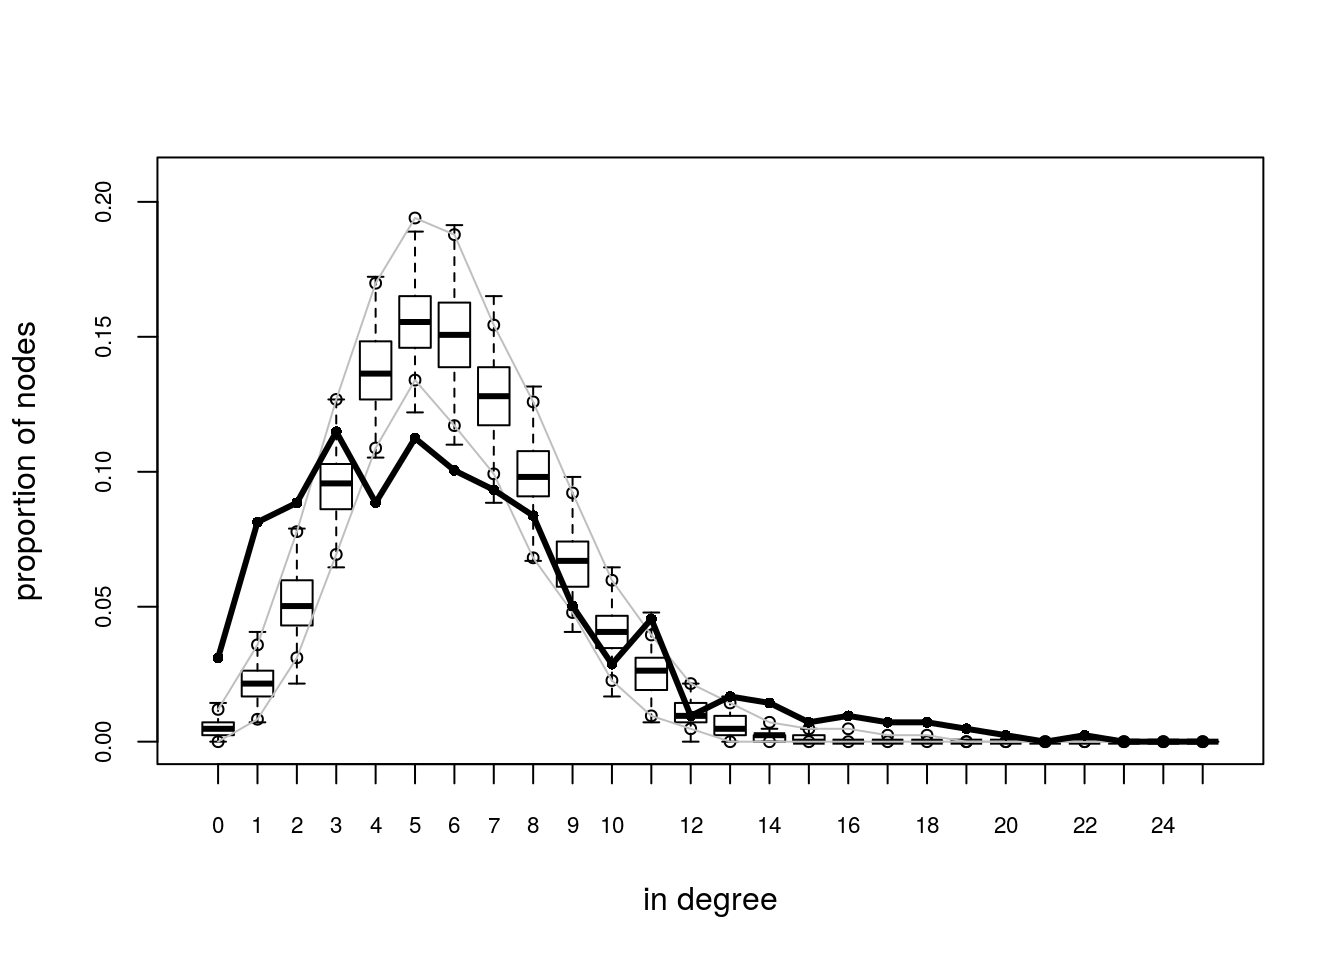
\includegraphics{appliedsnar_files/figure-latex/checking-gof-1.pdf}
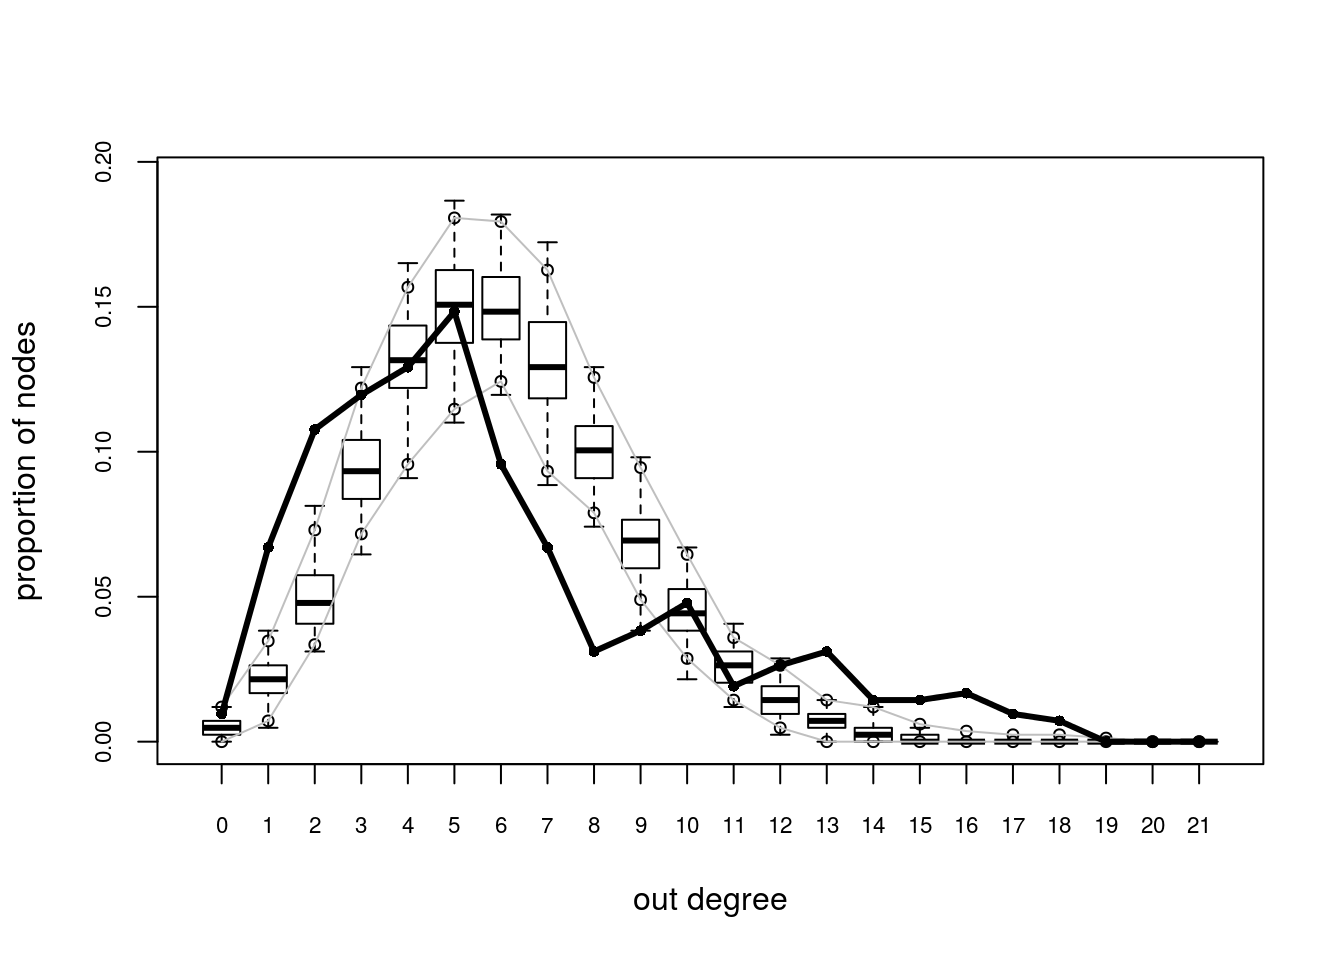
\includegraphics{appliedsnar_files/figure-latex/checking-gof-2.pdf}
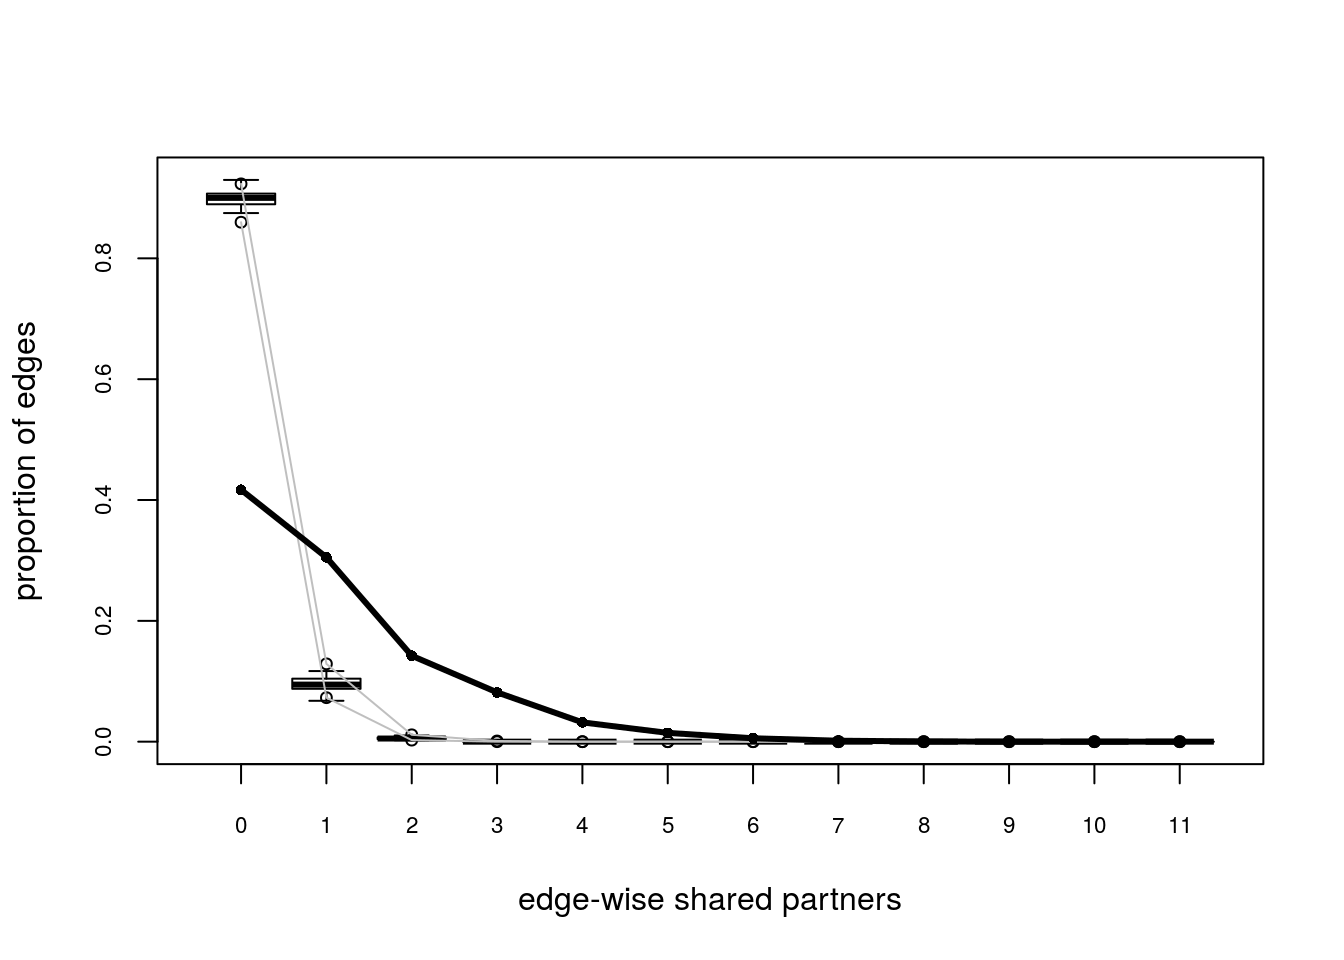
\includegraphics{appliedsnar_files/figure-latex/checking-gof-3.pdf}
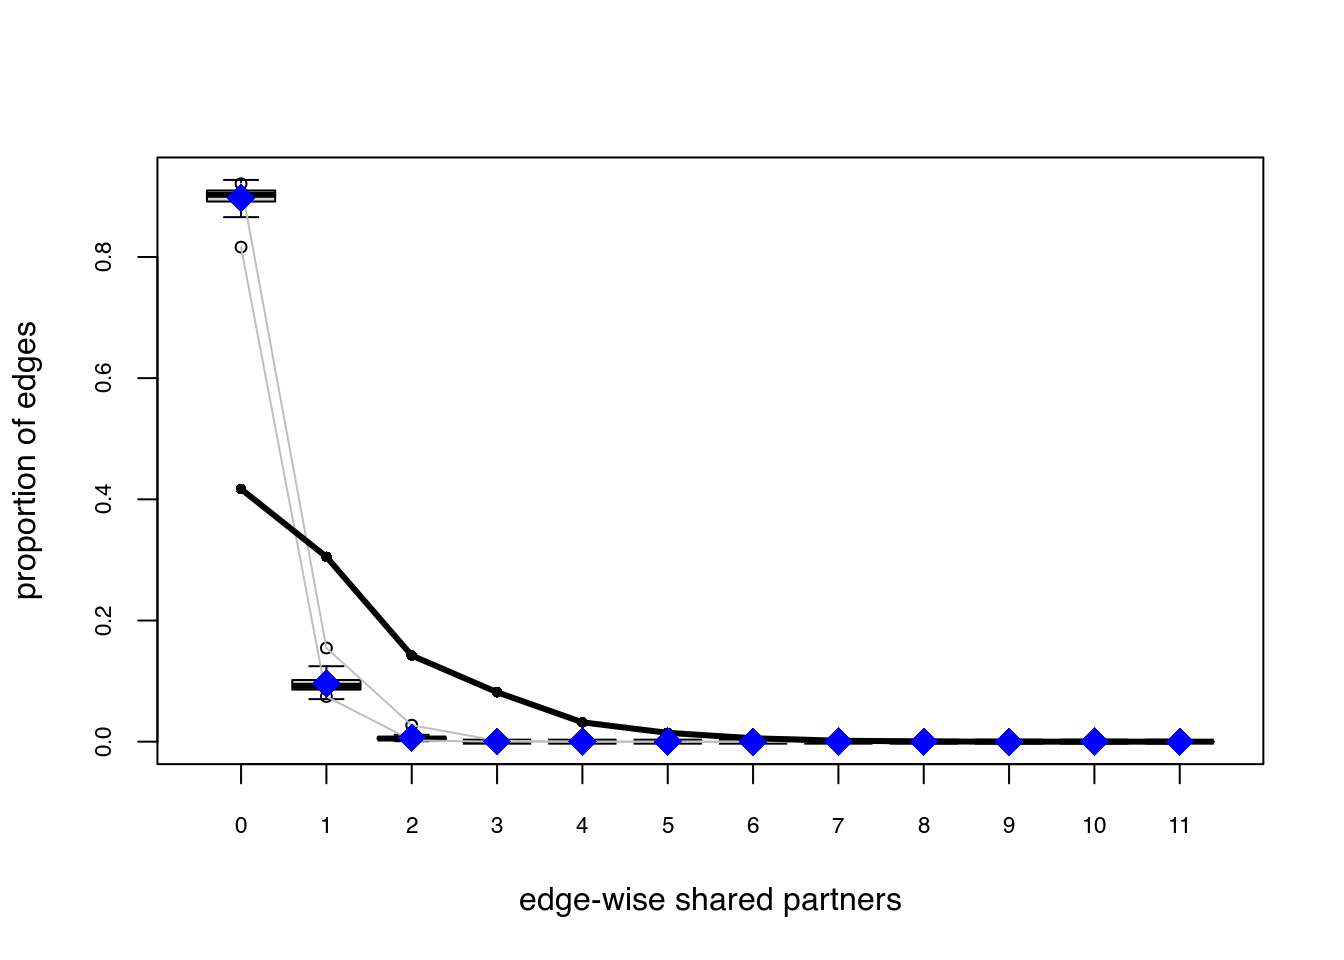
\includegraphics{appliedsnar_files/figure-latex/checking-gof-4.pdf}
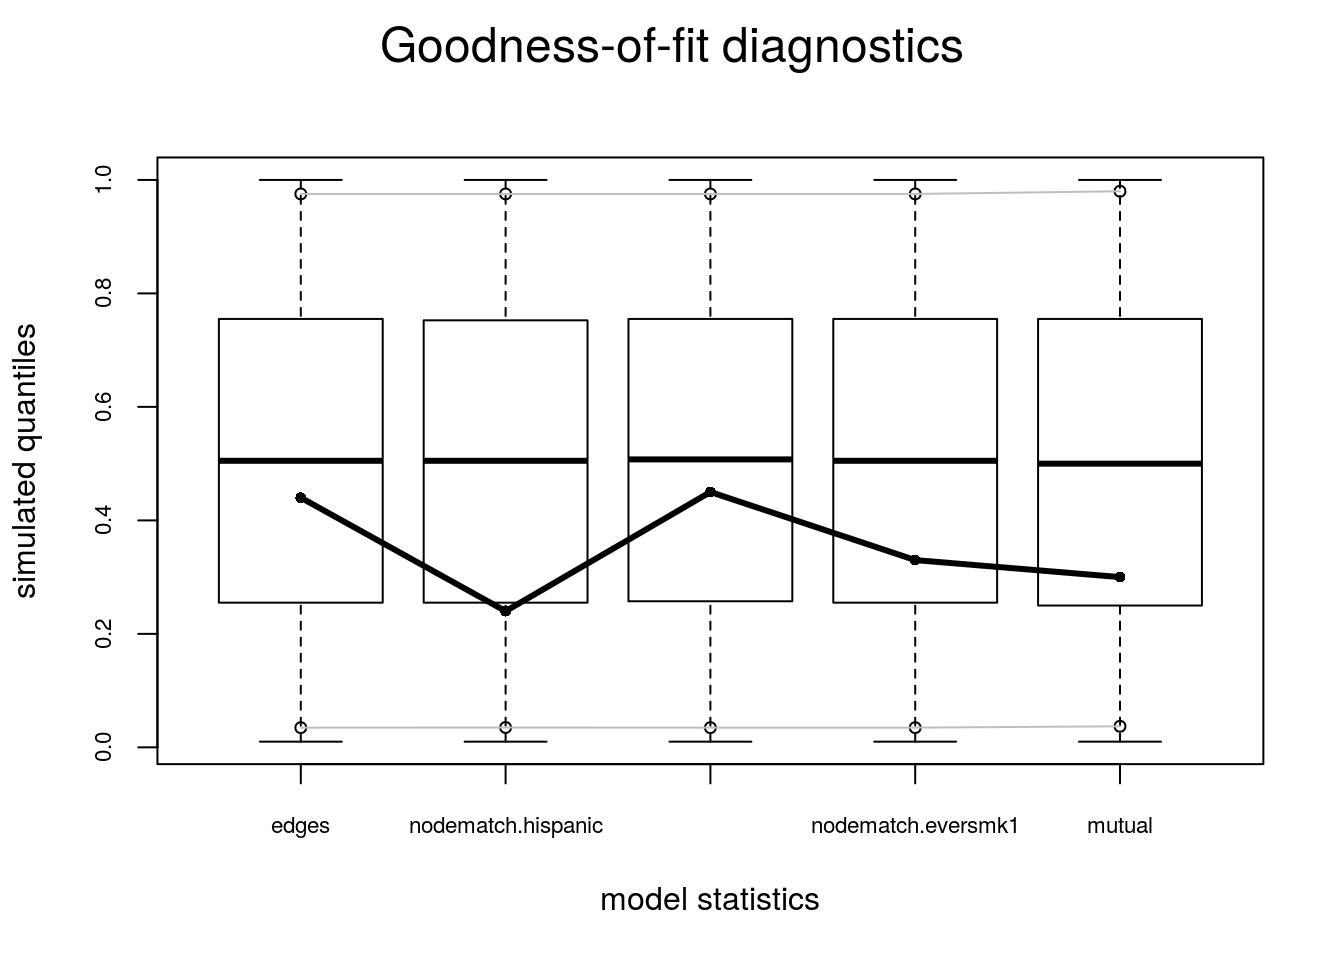
\includegraphics{appliedsnar_files/figure-latex/checking-gof-5.pdf}

\chapter{Final Words}\label{final-words}

We have finished a nice book.

\cleardoublepage 

\appendix


\chapter{Datasets}\label{datasets}

\hypertarget{sns-data}{\section{SNS data}\label{sns-data}}

\subsection{About the data}\label{about-the-data}

\begin{itemize}
\item
  This data is part of the NIH Challenge grant \# RC 1RC1AA019239
  ``Social Networks and Networking That Puts Adolescents at High Risk''.
\item
  In general terms, the SNS's goal was(is) ``Understand the network
  effects on risk behaviors such as smoking initiation and substance
  use''.
\end{itemize}

\subsection{Variables}\label{variables}

The data has a \emph{wide} structure, which means that there is one row
per individual, and that dynamic attributes are represented as one
column per time.

\begin{itemize}
\item
  \texttt{photoid} Photo id at the school level (can be repeated across
  schools).
\item
  \texttt{school} School id.
\item
  \texttt{hispanic} Indicator variable that equals 1 if the indivual
  ever reported himself as hispanic.
\item
  \texttt{female1}, \ldots{}, \texttt{female4} Indicator variable that
  equals 1 if the individual reported to be female at the particular
  wave.
\item
  \texttt{grades1},\ldots{}, \texttt{grades4} Academic grades by wave.
  Values from 1 to 5, with 5 been the best.
\item
  \texttt{eversmk1}, \ldots{}, \texttt{eversmk4} Indicator variable of
  ever smoking by wave. A one indicated that the individual had smoked
  at the time of the survey.
\item
  \texttt{everdrk1}, \ldots{}, \texttt{everdrk4} Indicator variable of
  ever drinking by wave. A one indicated that the individual had drink
  at the time of the survey.
\item
  \texttt{home1}, \ldots{}, \texttt{home4} Factor variable for home
  status by wave. A one indicates home ownership, a 2 rent, and a 3 a
  ``I don't know''.
\end{itemize}

During the survey, participants were asked to name up to 19 of their
school friends:

\begin{itemize}
\item
  \texttt{sch\_friend11}, \ldots{}, \texttt{sch\_friend119} School
  friends nominations (19 in total) for wave 1. The codes are mapped to
  the variable \texttt{photoid}.
\item
  \texttt{sch\_friend21}, \ldots{}, \texttt{sch\_friend219} School
  friends nominations (19 in total) for wave 2. The codes are mapped to
  the variable \texttt{photoid}.
\item
  \texttt{sch\_friend31}, \ldots{}, \texttt{sch\_friend319} School
  friends nominations (19 in total) for wave 3. The codes are mapped to
  the variable \texttt{photoid}.
\item
  \texttt{sch\_friend41}, \ldots{}, \texttt{sch\_friend419} School
  friends nominations (19 in total) for wave 4. The codes are mapped to
  the variable \texttt{photoid}.
\end{itemize}

\chapter*{References}\label{references}
\addcontentsline{toc}{chapter}{References}

\hypertarget{refs}{}
\hypertarget{ref-R-magrittr}{}
Bache, Stefan Milton, and Hadley Wickham. 2014. \emph{Magrittr: A
Forward-Pipe Operator for R}.
\url{https://CRAN.R-project.org/package=magrittr}.

\hypertarget{ref-R-intergraph}{}
Bojanowski, Michal. 2015. \emph{Intergraph: Coercion Routines for
Network Data Objects}. \url{http://mbojan.github.io/intergraph}.

\hypertarget{ref-R-igraph}{}
Csardi, Gabor, and Tamas Nepusz. 2006. ``The Igraph Software Package for
Complex Network Research.'' \emph{InterJournal} Complex Systems: 1695.
\url{http://igraph.org}.

\hypertarget{ref-R-ergm}{}
Handcock, Mark S., David R. Hunter, Carter T. Butts, Steven M. Goodreau,
Pavel N. Krivitsky, and Martina Morris. 2017. \emph{Ergm: Fit, Simulate
and Diagnose Exponential-Family Models for Networks}. The Statnet
Project (\url{http://www.statnet.org}).
\url{https://CRAN.R-project.org/package=ergm}.

\hypertarget{ref-R-statnet}{}
Handcock, Mark S., David R. Hunter, Carter T. Butts, Steven M. Goodreau,
Pavel N. Krivitsky, Skye Bender-deMoll, and Martina Morris. 2016.
\emph{Statnet: Software Tools for the Statistical Analysis of Network
Data}. The Statnet Project (\url{http://www.statnet.org}).
\url{CRAN.R-project.org/package=statnet}.

\hypertarget{ref-Hunter2008}{}
Hunter, David R., Mark S. Handcock, Carter T. Butts, Steven M. Goodreau,
and Martina Morris. 2008. ``ergm : A Package to Fit, Simulate and
Diagnose Exponential-Family Models for Networks.'' \emph{Journal of
Statistical Software} 24 (3).
doi:\href{https://doi.org/10.18637/jss.v024.i03}{10.18637/jss.v024.i03}.

\hypertarget{ref-R-texreg}{}
Leifeld, Philip. 2013. ``texreg: Conversion of Statistical Model Output
in R to LaTeX and HTML Tables.'' \emph{Journal of Statistical Software}
55 (8): 1--24. \url{http://www.jstatsoft.org/v55/i08/}.

\hypertarget{ref-Matloff2011}{}
Matloff, Norman. 2011. \emph{The Art of R Programming: A Tour of
Statistical Software Design}. No Starch Press.

\hypertarget{ref-R-coda}{}
Plummer, Martyn, Nicky Best, Kate Cowles, and Karen Vines. 2006. ``CODA:
Convergence Diagnosis and Output Analysis for Mcmc.'' \emph{R News} 6
(1): 7--11. \url{https://journal.r-project.org/archive/}.

\hypertarget{ref-R-foreign}{}
R Core Team. 2017. \emph{Foreign: Read Data Stored by 'Minitab', 'S',
'Sas', 'Spss', 'Stata', 'Systat', 'Weka', 'dBase', ...}
\url{https://CRAN.R-project.org/package=foreign}.

\hypertarget{ref-R-rex}{}
Ushey, Kevin, Jim Hester, and Robert Krzyzanowski. 2017. \emph{Rex:
Friendly Regular Expressions}.
\url{https://CRAN.R-project.org/package=rex}.

\hypertarget{ref-R-stringr}{}
Wickham, Hadley. 2017. \emph{Stringr: Simple, Consistent Wrappers for
Common String Operations}.
\url{https://CRAN.R-project.org/package=stringr}.

\hypertarget{ref-R-readxl}{}
Wickham, Hadley, and Jennifer Bryan. 2017. \emph{Readxl: Read Excel
Files}. \url{https://CRAN.R-project.org/package=readxl}.

\hypertarget{ref-R-tidyr}{}
Wickham, Hadley, and Lionel Henry. 2017. \emph{Tidyr: Easily Tidy Data
with 'Spread()' and 'Gather()' Functions}.
\url{https://CRAN.R-project.org/package=tidyr}.

\hypertarget{ref-R-dplyr}{}
Wickham, Hadley, Romain Francois, Lionel Henry, and Kirill Müller. 2017.
\emph{Dplyr: A Grammar of Data Manipulation}.
\url{https://CRAN.R-project.org/package=dplyr}.

\hypertarget{ref-R-readr}{}
Wickham, Hadley, Jim Hester, and Romain Francois. 2017. \emph{Readr:
Read Rectangular Text Data}.
\url{https://CRAN.R-project.org/package=readr}.


\end{document}
